\documentclass[10pt, landscape]{article}
\usepackage[scaled=0.92]{helvet}
\usepackage{multicol}
\usepackage{calc}
\usepackage{ifthen}
\usepackage[landscape]{geometry}
%\usepackage{hyperref}

\usepackage{newtxtext} 

%for strikeout
\usepackage{ulem}

%For editing parbox
\usepackage[table]{xcolor}
%For editing itemise margins, reduce iterm separaion and list separation
\usepackage{enumitem}
% For math
\usepackage{amsmath,amsthm,amsfonts,amssymb}

%For pictures / figures
\usepackage{color,graphicx,overpic}
\graphicspath{ {./images/} }

%\usepackage{newtxtext} 
%\usepackage{amssymb}
%\usepackage[table]{xcolor}
%\usepackage{vwcol}
%\usepackage{tikz}
%\usepackage{wrapfig}
%\usepackage{makecell}

\pdfinfo{
  /Title (CS2106-notes.pdf)
  /Creator (Ger Teck)
  /Author (Ger Teck)
  /Subject ()
  /Keywords (tex)}

%% Margins for PAPER

% This sets page margins to .5 inch if using letter paper, and to 1cm
% if using A4 paper. (This probably isn't strictly necessary.)
% If using another size paper, use default 1cm margins.
\ifthenelse{\lengthtest { \paperwidth = 11in}}
	{ \geometry{top=.3in,left=.3in,right=.3in,bottom=.3in} }
	{\ifthenelse{ \lengthtest{ \paperwidth = 297mm}}
		{\geometry{top=0.5cm,left=0.5cm,right=0.5cm,bottom=0.5cm} }
		{\geometry{top=0.5cm,left=0.5cm,right=0.5cm,bottom=0.5cm} }
	}

% Turn off header and footer
\pagestyle{empty}
% for tight centres (less spacing)
\newenvironment{tightcenter}{%
  \setlength\topsep{0.5pt}
  \setlength\parskip{0.5pt}
  \begin{center}
}{%
  \end{center}
}

% Redefine section commands to use less space
\makeatletter
\renewcommand{\section}{\@startsection{section}{1}{0mm}%
                                {-1ex plus -.5ex minus -.2ex}%
                                {0.5ex plus .2ex}%x
                                {\normalfont\large\bfseries}}
\renewcommand{\subsection}{\@startsection{subsection}{2}{0mm}%
                                {-1explus -.5ex minus -.2ex}%
                                {0.5ex plus .2ex}%
                                {\normalfont\normalsize\bfseries}}
\renewcommand{\subsubsection}{\@startsection{subsubsection}{3}{0mm}%
                                {-1ex plus -.5ex minus -.2ex}%
                                {1ex plus .2ex}%
                                {\normalfont\small\bfseries}}
% change font
%\renewcommand{\familydefault}{\sfdefault}
%\renewcommand\rmdefault{\sfdefault}
\linespread{1.05}

\makeatother

% Define BibTeX command
\def\BibTeX{{\rm B\kern-.05em{\sc i\kern-.025em b}\kern-.08em
    T\kern-.1667em\lower.7ex\hbox{E}\kern-.125emX}}

% Don't print section numbers
\setcounter{secnumdepth}{0}

\setlength{\parindent}{0pt}
\setlength{\parskip}{0pt plus 0.5ex}

%% this changes all items (enumerate and itemize, reduce margins) ITEMIZE SEPARATION HERE
\setlength{\leftmargini}{0.5cm}
\setlength{\leftmarginii}{0.5cm}
\setlist[itemize,1]{leftmargin=2mm,labelindent=1mm,labelsep=1mm, itemsep = 0mm}
\setlist[itemize,2]{leftmargin=4mm,labelindent=1mm,labelsep=1mm, itemsep = 0mm}

% For Code Blocks
\usepackage{xcolor}
\usepackage{listings}

\lstdefinestyle{mystyle}{
	backgroundcolor=\color{gray!25!white},
	basicstyle=\scriptsize,
	numbers=none,    %or = none or left
	showstringspaces=false,
	breaklines=true,
	breakatwhitespace=false,                  
	captionpos=b,                    
	keepspaces=true,                                 
	numbersep=5pt,                  
	showspaces=false,                
	showtabs=false,                  
	tabsize=2,
 }
%Helpful:
%[linewidth = 1.0 \linewidth]
%\lstinline{}
% use \code{} for \lstinline with colorbox.
\newcommand{\code}[1]{\colorbox{gray!25!}{\lstinline|#1|}}
\lstset{style=mystyle}

%\begin{lstlisting} [linewidth = 1.0 \linewidth],
% code here
%\end{lstlisting}

%itemsep = 0mm
%\setlist{nosep}

% -------------------------------------------------------------------------------

% START OF DOCUMENT HERE

\begin{document}
\raggedright
\footnotesize
\begin{multicols*}{3}

% multicol parameters
% These lengths are set only within the two main columns
%\setlength{\columnseprule}{0.25pt}
\setlength{\premulticols}{1pt}
\setlength{\postmulticols}{1pt}
\setlength{\multicolsep}{1pt}
\setlength{\columnsep}{2pt}

%% DOCUMENT NAME HERE
\begin{center}
     \Large{\textbf{CS2106 Intro Op. Systems Notes}} \\
\end{center}
AY23/24 Sem 2, github.com/gerteck


\section{1. Introduction}
\textbf{Course objectives:} Introduces basic concepts in operating systems. Focusing on: \\
- OS structure and architecture, process management, memory management, file management and OS protection mechanism. \\
- Identify and understand major functionalities of modern operating systems. \\
- Extend and apply the knowledge in future courses.

\textbf{Supplementary Text}: Modern Operating System (5th Edition), by Andrew S. Tanenbaum, Pearson, 2023.

\subsection{Learning Outcomes}
\begin{itemize}
	\item Understand how an \textbf{OS manages computational resources for multiple users and applications, and the impact on application performance}
	\item Appreciate the \textbf{abstractions and interfaces provided by OS}
	\item Write \textbf{multi-process / thread programs} and avoid common pitfalls such as \textbf{deadlocks, starvation and race conditions.}
	\item Write system programs that utilizes \textbf{POSIX} syscall for process, memory and I/O management.
	\item Self-learn and explore advanced OS topics.
	\item Understand important design principles in complex systems.
\end{itemize}

Areas to focus on: Try to understand how things are running in parallel, since we naturally think sequentially. Secondly, how we can manage memory and how they combine and interact (in strange ways), synchronization.

\subsection{Operating System OS}
An OS is a program that acts as an intermediary between a computer user and the computer hardware. Motivation for OS:
\begin{itemize}
\item Manage resources and coordination. (Resource Allocator: Process synchronization, resource sharing)
\item Simplify programming (Abstraction of hardware / hardware virtualization, convenient services)
\item Enforce usage policies
\item Security and protection
\item User Program Portability (across different hardware)
\item Efficiency (Optimize for particular usage and hardware).
\end{itemize}

\textbf{Kernel Mode}: Complete access to all hardware resources. \\
\textbf{User Mode}: Limited / Controlled access to hardware resources.

\hspace{0.5cm}

\centerline{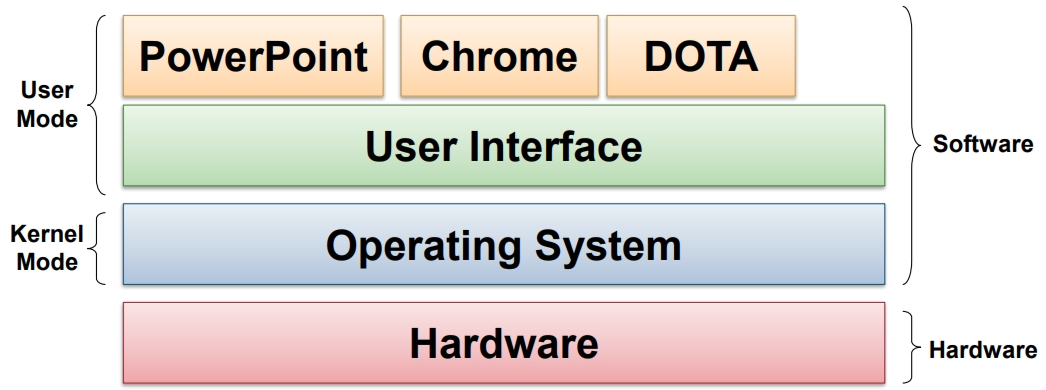
\includegraphics[width=0.5\linewidth]{highlevelOS}}

\subsubsection{Generic OS Components}
\centerline{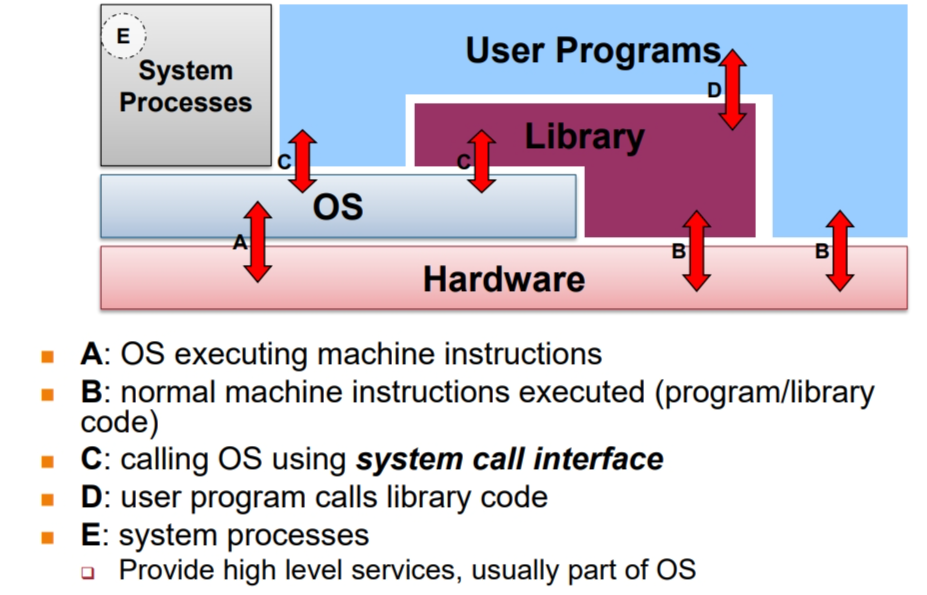
\includegraphics[width=0.7\linewidth]{genericOS}}
\begin{itemize}
\item OS is known as the \textbf{kernel}. \\
		Program that deals with hardware issues, provide system call interface and special code for interrupt handlers, device drivers.
\item Kernel code is different from normal programs: \\
		No use of system call in kernel code, can't use normal libraries, no normal I/O (must do I/O itself).
\item \textbf{Implementing OS}: Historically in assembly/machine, now in HLLs (C, C++). Heavily hardware architecture dependent. Challenges include complexity, debugging, codebase size.
\end{itemize}

\subsubsection{OS Structures}
\textbf{Monolithic OS}: One Big program.
\begin{itemize}
\item Well understood, good performance, but highly coupled components (everything running in kernel mode) and usually devolved into very complicated internal structure.
\end{itemize}

\textbf{Microkernel OS}: 
\begin{itemize}
\item Kernel is very small and clean, only providing basic and essential facilities.
\item Inter-Process Communication \textbf{(IPC)}, Address space management, Thread management etc.
\item Higher level services are built on top of basic facilities, run as server process \textit{outside} of OS, use IPC to communicate.
\item Kernel is more robust and extendible, better isolation and protection between kernel and high level services. But, lower performance. (Latency)
\end{itemize}
\centerline{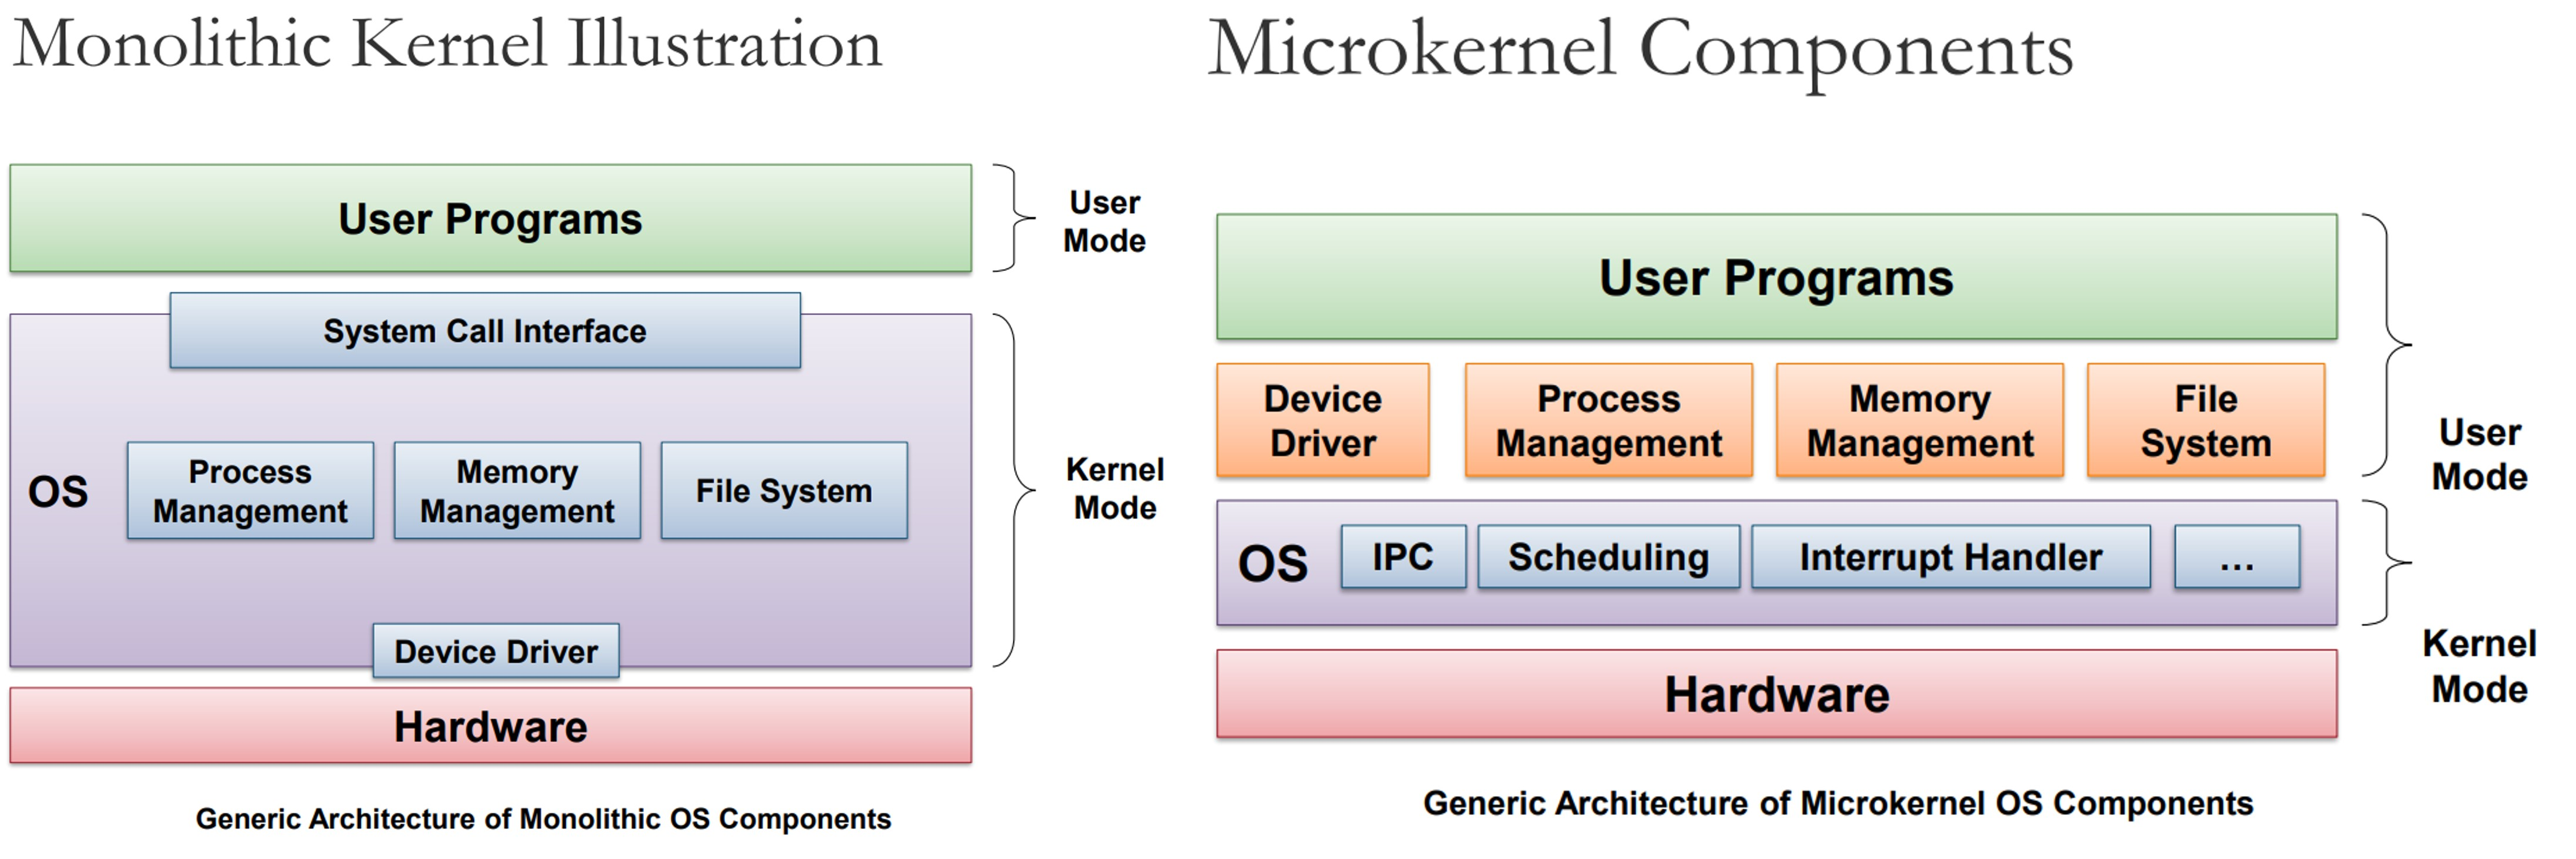
\includegraphics[width=0.95\linewidth]{OSstructure}}

\textbf{Other OS Structure}
\begin{itemize}
\item \textbf{Layered Systems}: Generalization of monolithic system, organize components into hierarchy of layers. Lowest is hardware, highest is user interface.
\item \textbf{Client-Server Model}: Variation of microkernel. Two classes of processes: Client p. request service from server process, server process built on top of microkernel. Client \& Server process can be on separate machine.
\end{itemize}

\subsubsection{Virtual Machines}
\begin{itemize}
\item \textbf{Motivation}: OS assumes total control of hardware, making it hard to run several OS on same hardware at same time. OS is also hard to debug / monitor, hard to observe working of OS, test potentially destructive implementation.
\item \textbf{Virtual Machine}: Software emulation of hardware. 
\item \textbf{Virtualization of underlying hardware}: Illusion of complete hardware to level above. (Memory, CPU etc.) Normal OS can then run on top of virtual machine. Aka \textbf{Hypervisor}. 
	\begin{itemize}
	\item \textbf{Type 1 Hypervisor}: Provides individual virtual machines to guest OSes (e.g. IBM VM/370)
	\item \textbf{Type 2 Hypervisor}: Runs in host OS, Guest OS runs inside Virtual Machine, (e.g. VMware)
	\end{itemize}
\end{itemize}
\centerline{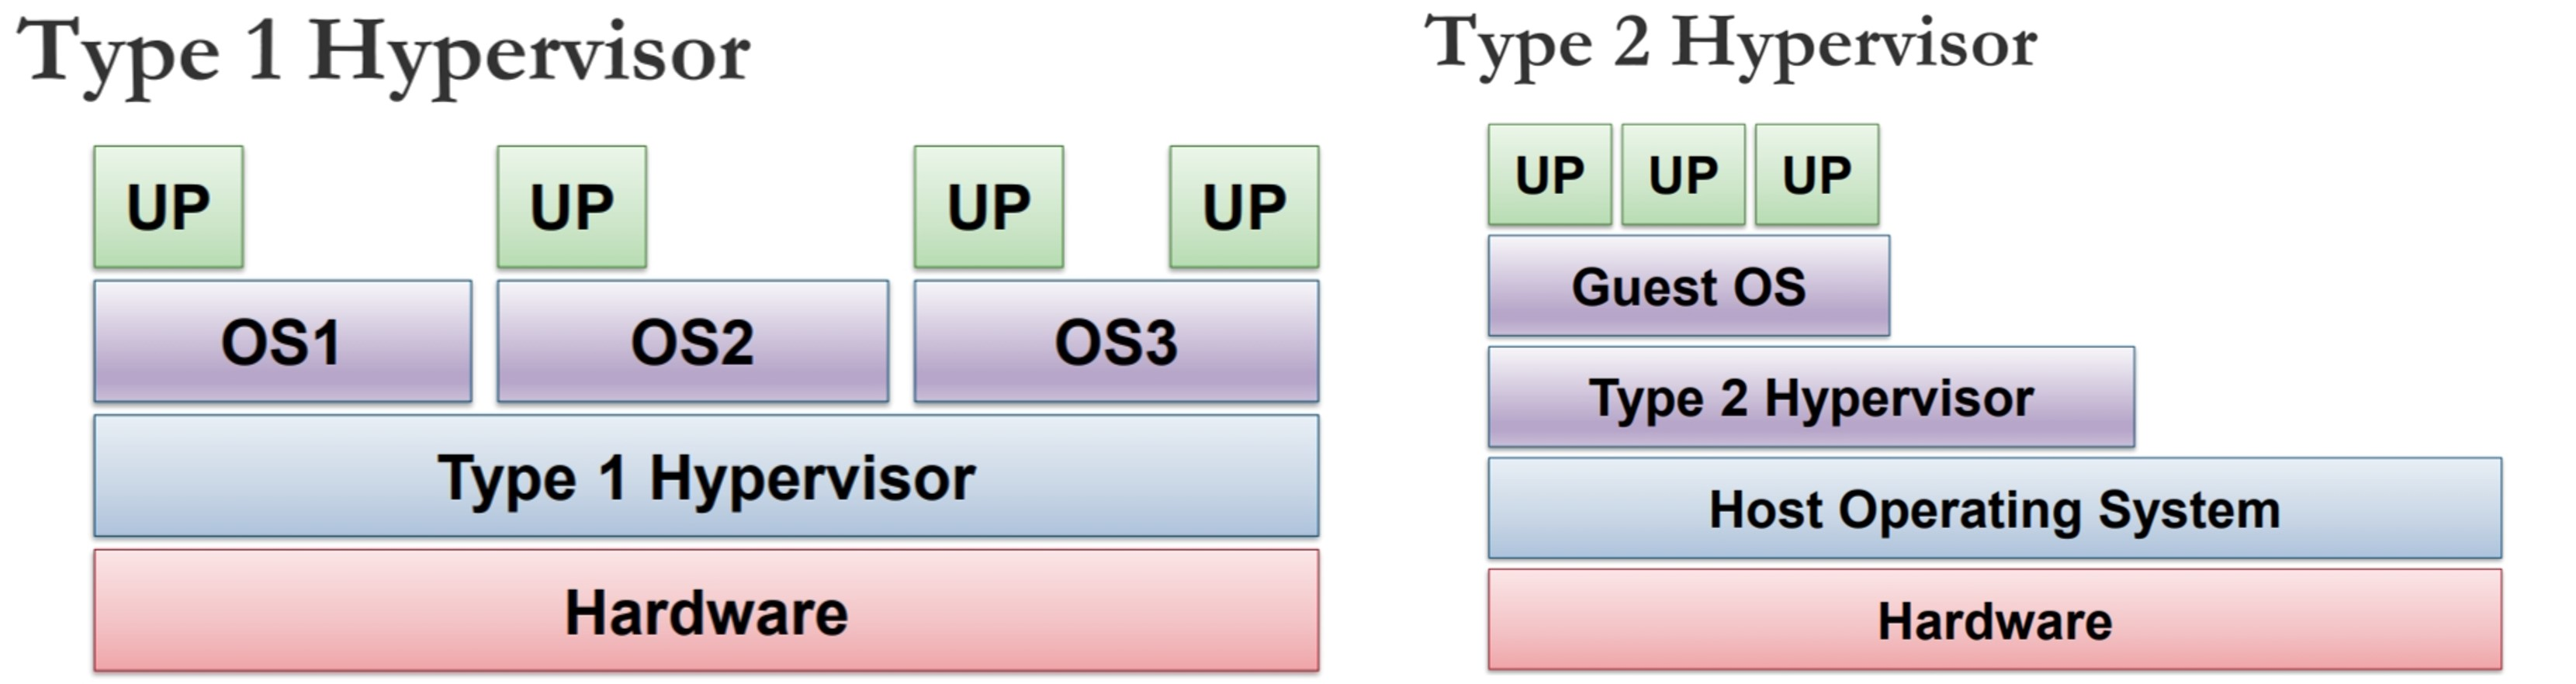
\includegraphics[width=0.9\linewidth]{hypervisor}}

\section{- Upcoming Topics -}
\textbf{OS Process Management}: As OS (to maximise efficiency hardware resources), to be able to switch from running one program to the other (share hardware, e.g. CPU), requires information regarding execution of A stored, and A's information replaced with B's information to run. (E.g. the registers in CPU replaced)
\begin{itemize}
	\item \textbf{2. Process Abstraction}: Info describing executing program
	\item \textbf{3. Process Scheduling}: Deciding which process gets to execute
	\item \textbf{4. Inter-Process Communication}: Passing information between processes (tough)
	\item \textbf{5. Threads + Synchronization}: Alternative to Process (Light-weight process aka Thread)
	\item \textbf{6. Memory Management}
	\item \textbf{7. Disjoint Memory Management}
	\item \textbf{8. File System Management}
	\item \textbf{9. File System Implementation}
\end{itemize}


\null \null \null \null
\null \null \null \null

\columnbreak


\section{2. Process Abstraction}
To switch programs, requires information of both programs. Hence, we need abstraction to describe running program, aka \textbf{process}.
\begin{itemize}
\item \textbf{(Process / Task / Job)} is a dynamic abstraction for executing program. 
\item It is info required to describe a \textit{running program}: \\
- Memory Context (Code/Text, Data, Stack, Heap),\\
- Hardware Context (Register/PC, Stack/Frame Pointer), \\
- OS Context (Process Properties (PID, State), Resources Used).
\end{itemize}

\subsubsection{Computer Organization (Recap)}
\begin{itemize}
\item \textbf{Components}: Memory, Cache, Fetch Unit (Loads instruction, location indicated by special register \textbf{PC}.)
\item \textbf{Functional Units} (Carry out instruction execution, dedicated to diff. instr. type) (CS2100 looked at INT func. unit)
\item Registers (Internal storage, fastest access speed). \\
- \textbf{GPR}: General Purpose Register, accessible by user program / compiler. \\
- \textbf{Special Registers}: PC, Stack/Frame Pointer, PSW etc.
\item \textbf{Binary Executable File}: file in machine language (built by compiler) for specific processor: \\
- Executable (binary) consists two major components: Instr. (Text) \& Data \\
- When under execution, more info: Memory, Hardware, OS context.	
\end{itemize}
\centerline{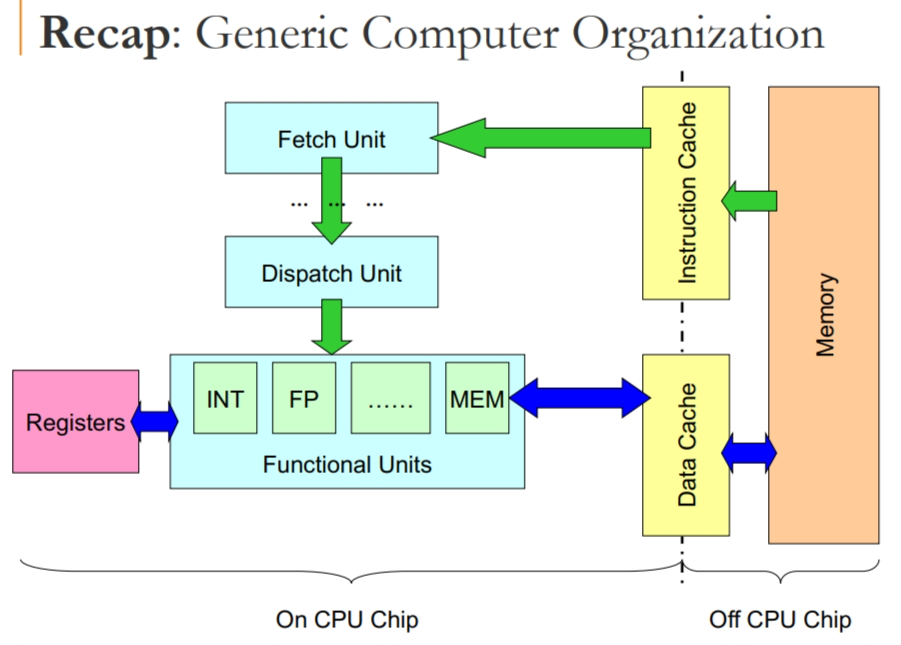
\includegraphics[width=0.6\linewidth]{computerOrg}}

\subsection{Memory Context for Function Call (Stack Memory)}
\textbf{Memory Context Challenges of Functional Calls:}
\begin{itemize}
\item Control Flow Issues: Need to jump to function body, resume after, need to store PC of caller.
\item Data Storage Issues: Need to pass params to function, capture return result, may need declare local variables.
\item Require region of memory dynamically used by function invocations.
\end{itemize}
Hence, portion of memory space used as \textbf{stack memory} that stores executing function using \textbf{stack frame}, which includes usage of \textit{Stack Pointer, Frame Pointer}.

\subsubsection{Stack Memory Region}
\begin{itemize}
\item \textbf{Memory region to store information function invocation.}
\item \textbf{Stack Frame}: Describes information of function invocation.
\item Stack frame added on top when function is invoked, stack "grows", removed from top when function call ends, stack "shrinks".
\item Stack Frame contains return PC address of caller, arguments for function, storage for local variable, etc.
\item \textbf{Stack Pointer}: Indicates top of stack region (first unused memory location). Usually indicated in specialized register.
\end{itemize}


\subsubsection{Function Call Convention: Stack Frame Setup / Teardown}
There are different ways to setup stack frame, known as function call convention, differences about (info stored in frame, which portion of stack frame prepared \& cleared by caller / callee etc). Dependent on hardware \& programming language. \\
\medskip
\textbf{Example Scheme:}
\centerline{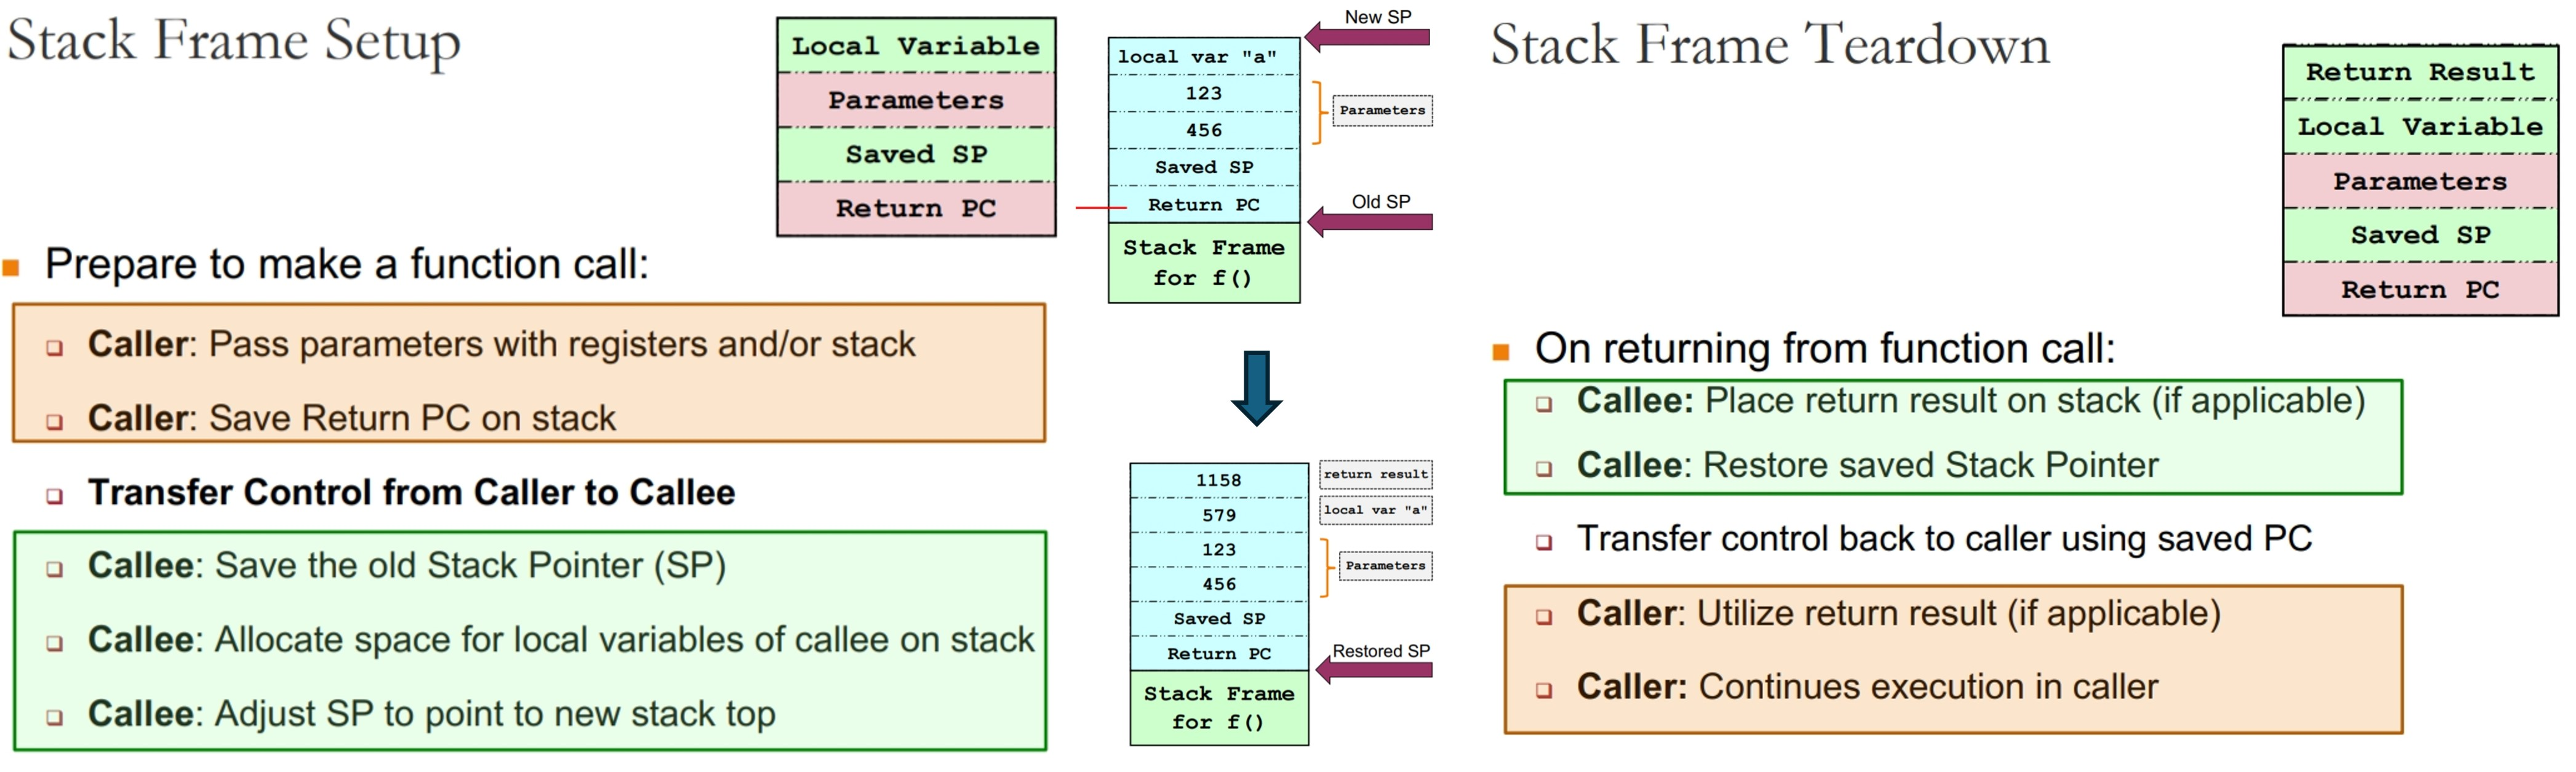
\includegraphics[width=1\linewidth]{stackSetupTeardown}}
\smallskip
\centerline{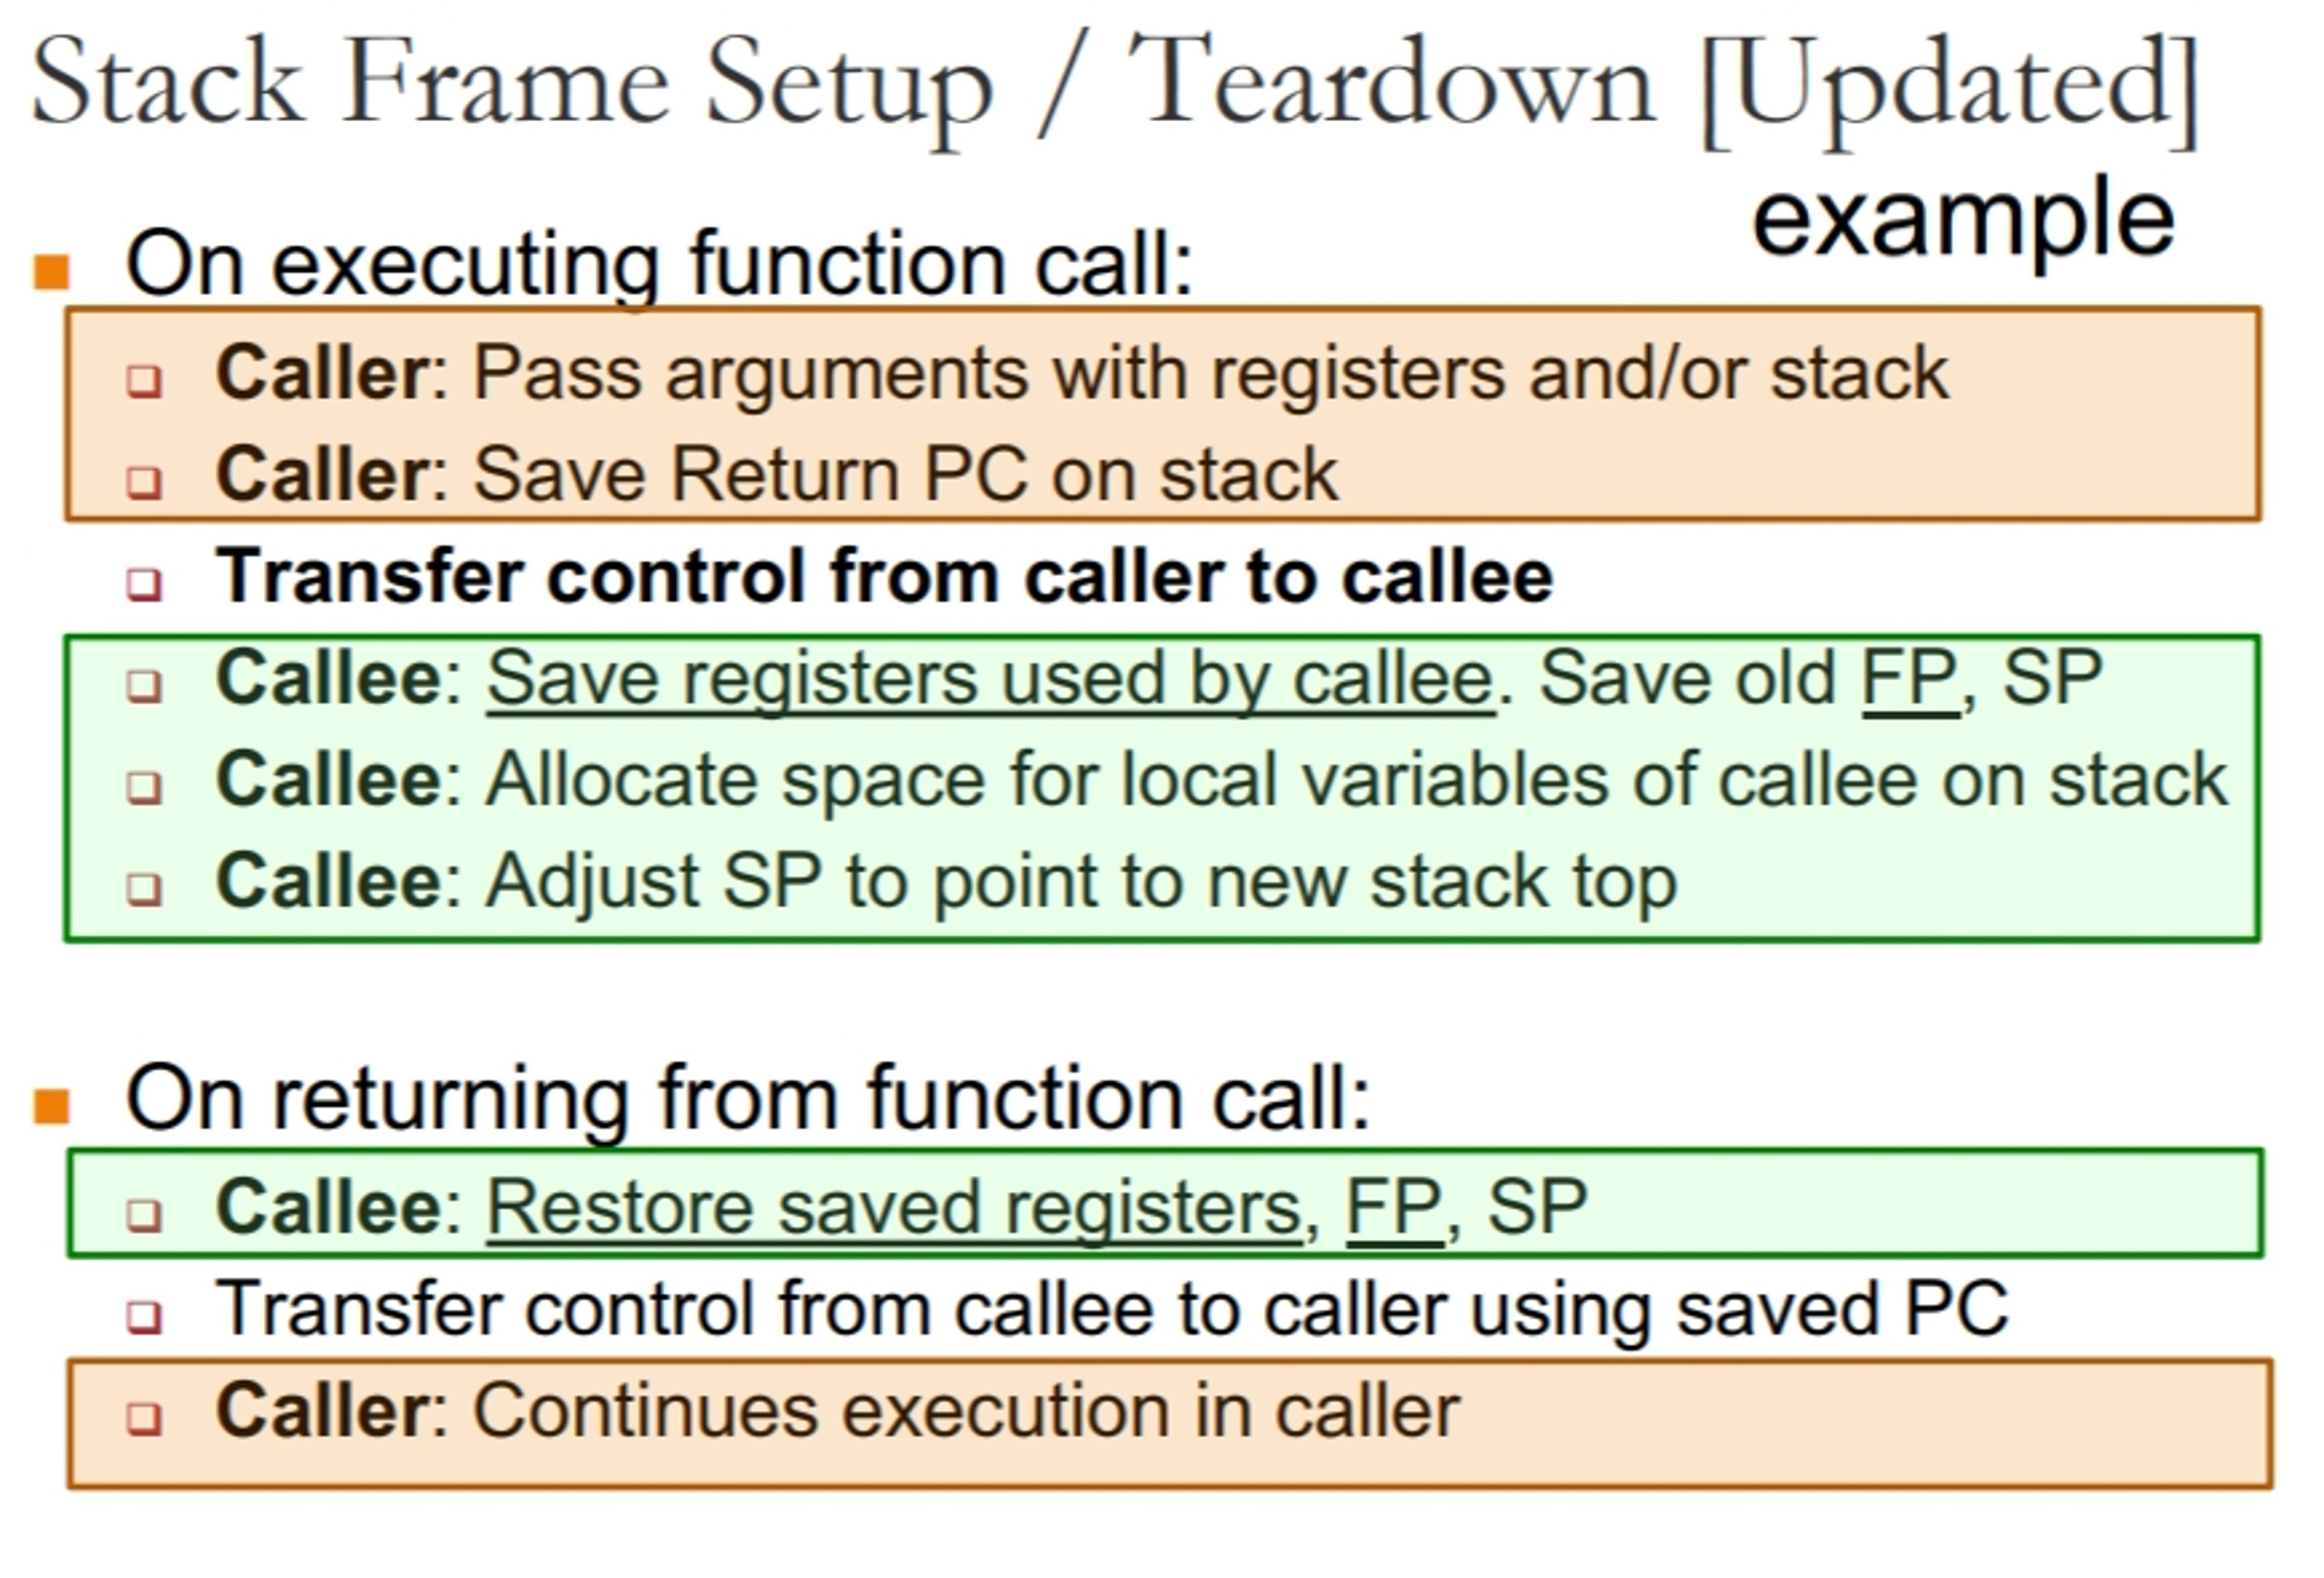
\includegraphics[width=0.45\linewidth]{stackSetupTeardown2}}

\subsubsection{Stack Frame: Other Information}
\textbf{Frame Pointer}
\begin{itemize}
\item To facilitate access of various stack frame items. As stack pointer hard to use as it can change, some processors provide dedicated register Frame Pointer.
\item Frame Pointer points to fixed location in stack frame, other items accessed as displacement from frame pointer, usage of FP is platform dependent.
\end{itemize}

\textbf{Saved Registers}
\begin{itemize}
\item Since number of GPR limited, when GPR exhausted, use memory to temp. hold GPR values for reuse.
\item \textbf{Known as Register Spilling}. Function can spill registers it intends to use before function starts, then restore registers at end of function.
\end{itemize}

\centerline{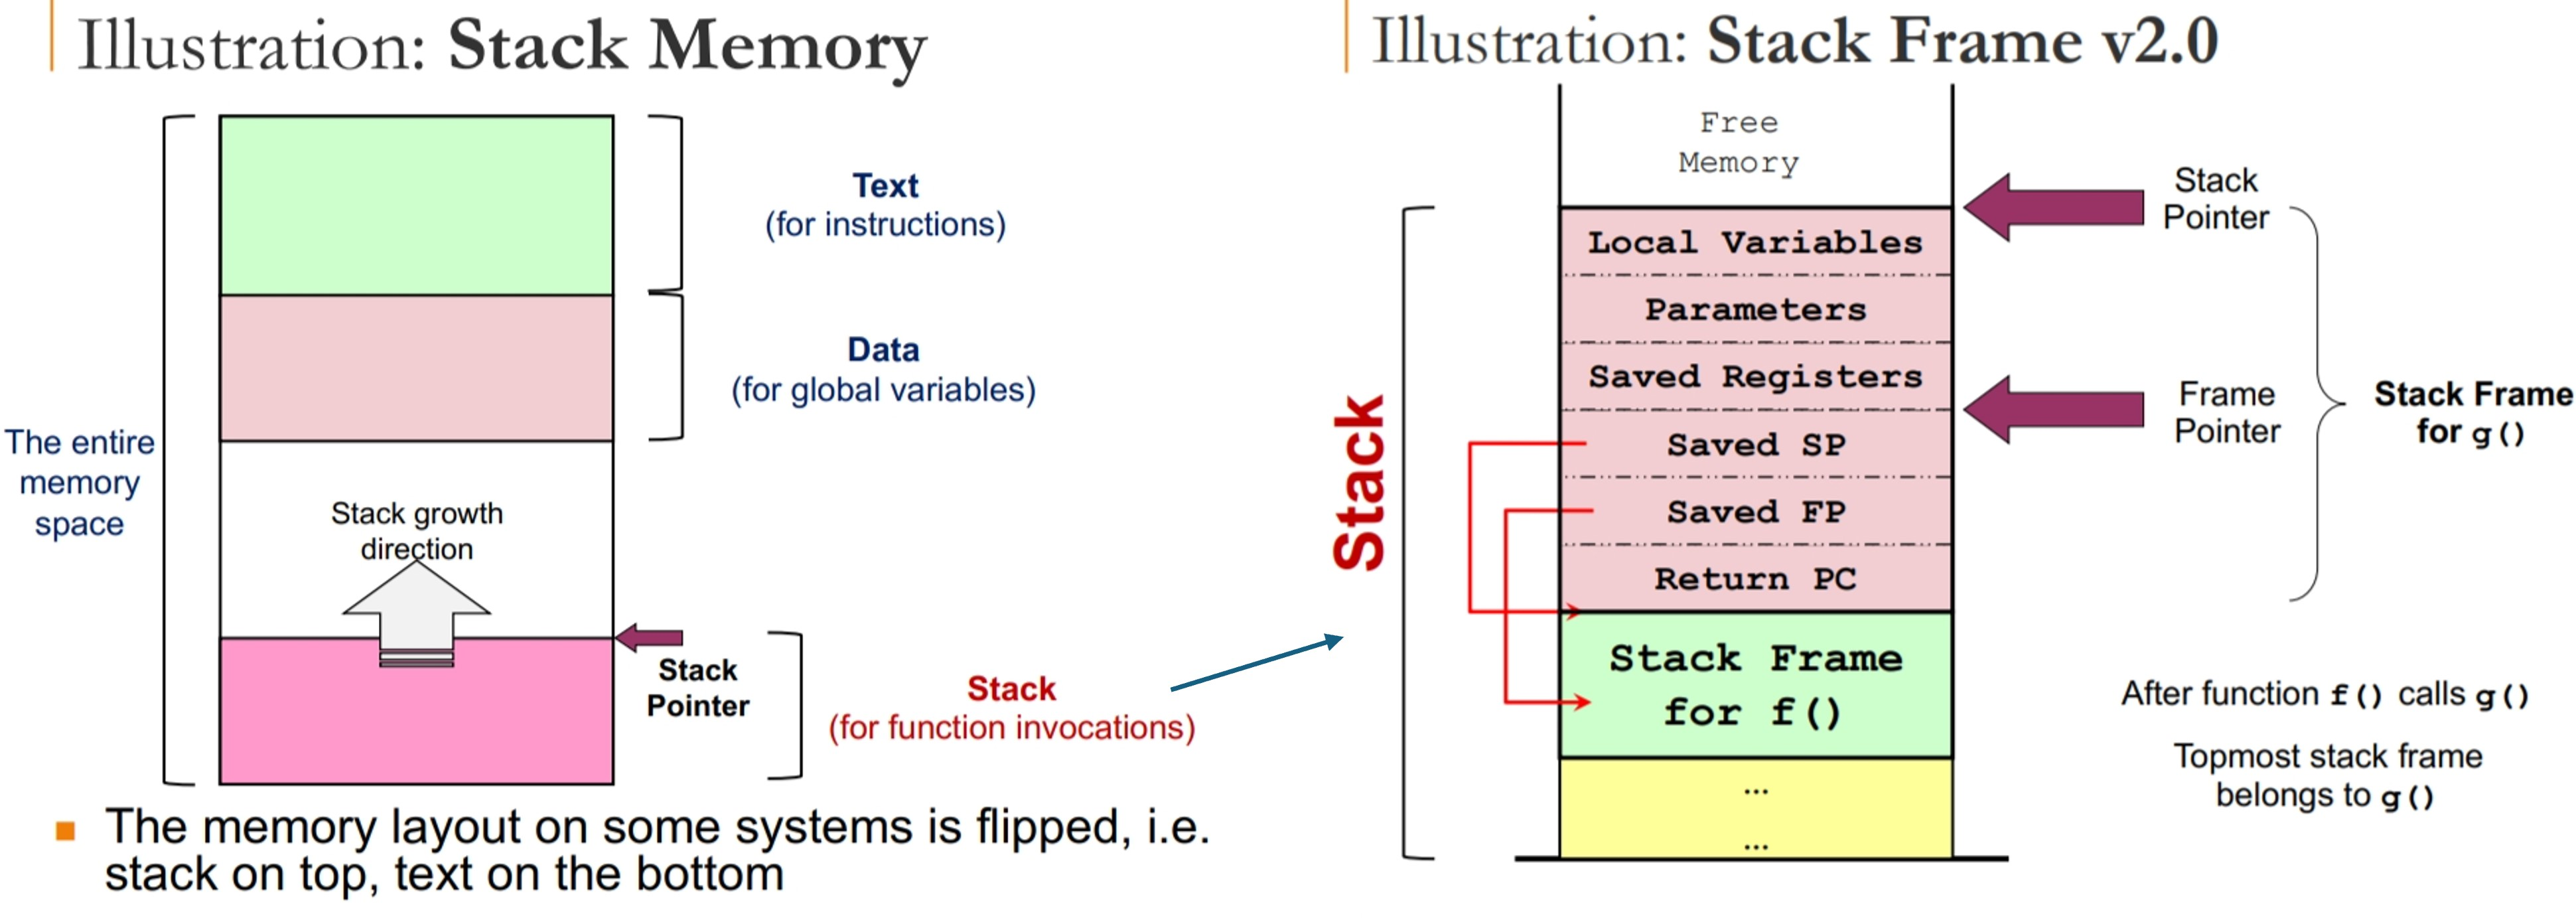
\includegraphics[width=1\linewidth]{stackMemory}}

\subsection{Memory Context for Dynamically Allocated Mem. (Heap)}
Most programming languages allow dynamically allocated memory, i.e. acquire memory space during execution time.
\begin{itemize}
\item In C, \code{malloc()} function call, while C++ / Java: \code{new} keyword.
\item Cannot place in \textit{Data region}, as allocated at runtime, size not known during compilation.
\item Cannot place in \textit{Stack region}, as no definite deallocation time, cannot be freed by garbage collector.
\item Solution: Set up separate \textbf{Heap Memory Region}
\end{itemize}

\columnbreak

\subsubsection{Heap Memory}
\begin{itemize}
\item Managing heap memory trickier due to variable size, variable allocation / deallocation timing.
\item Common situation where heap memory alloc/dealloc creating "holes" in memory. Free memory block squeezed between occupied memory blocks.
\item Covered in memory management.
\end{itemize}
\centerline{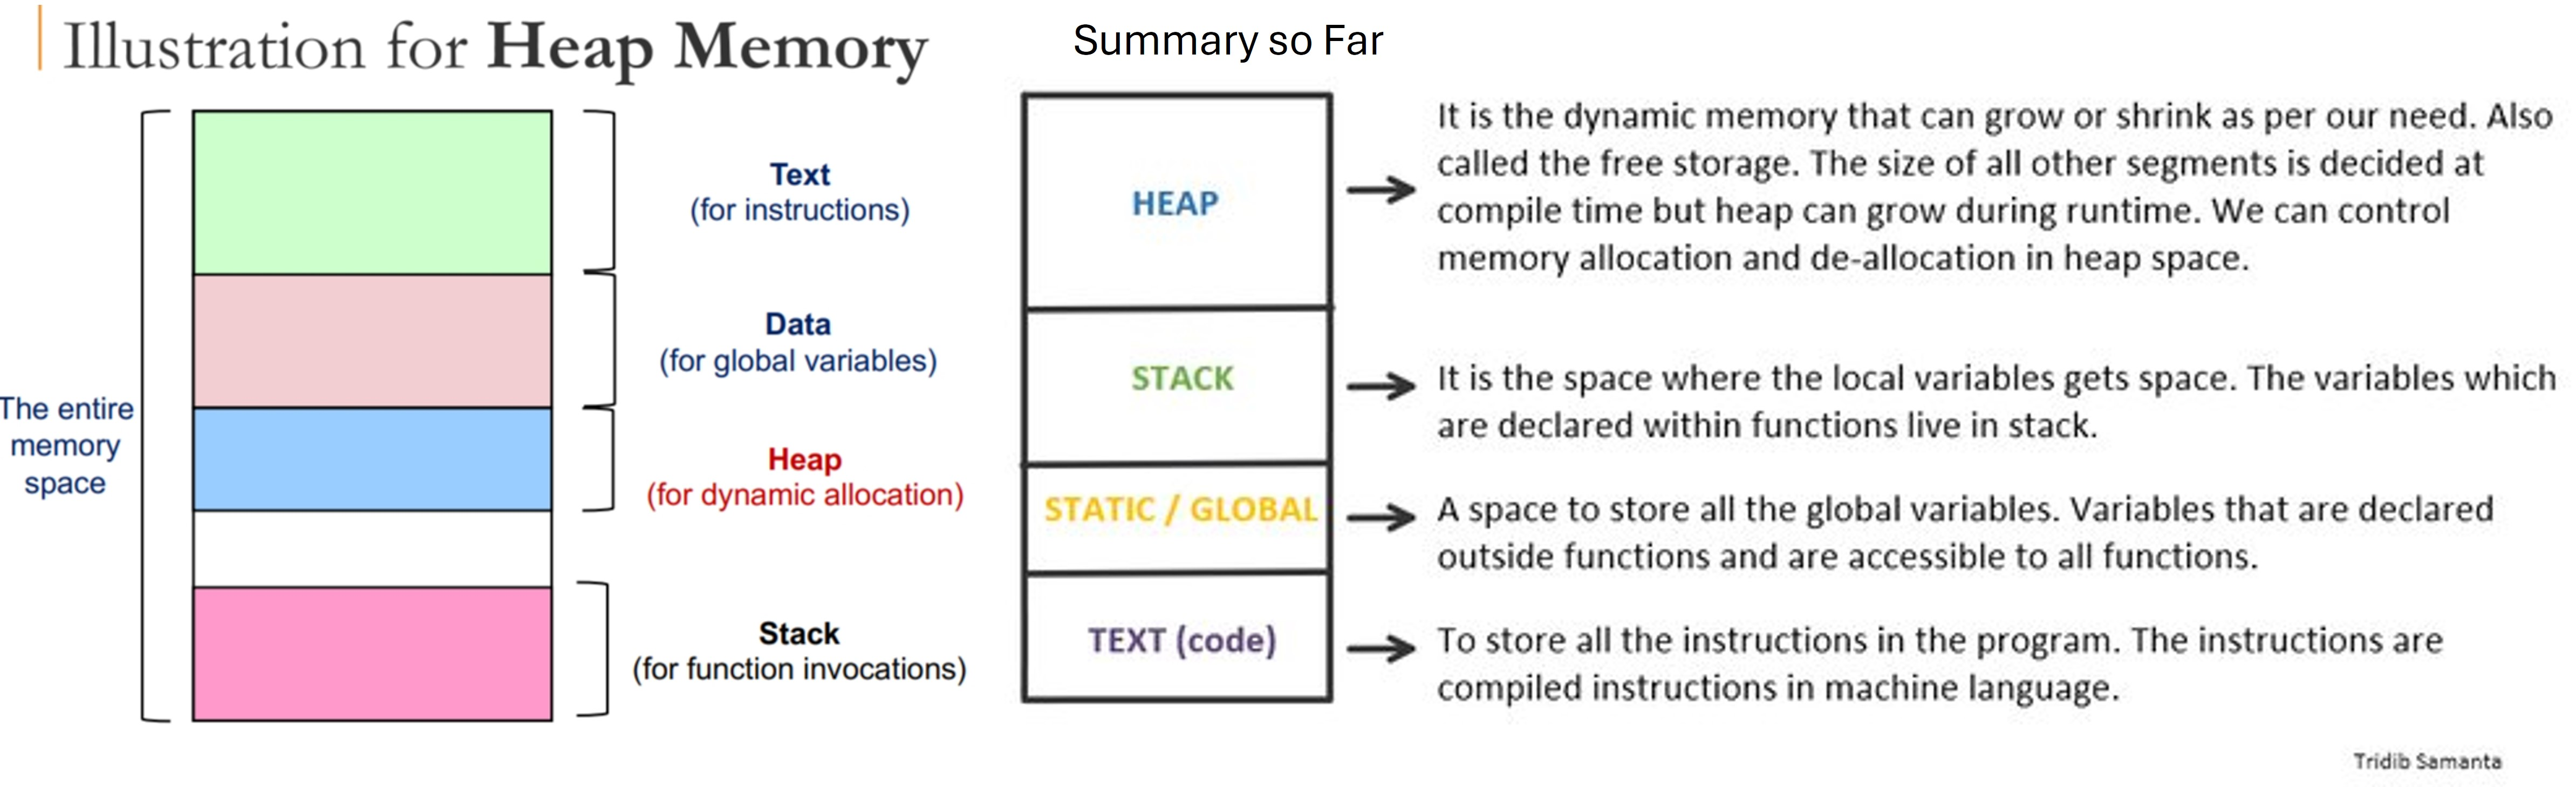
\includegraphics[width=1\linewidth]{heapMemory}}


\subsection{OS Context: Process ID, Process State}
\textbf{Process Identification}:
\begin{itemize}
\item \textbf{Process ID}: To distinguish processes from each other (Just a number, unique among processes)
\item PIDs are OS dependent as well, including if PIDs reused, if limits maximum no. of processes or any PIDs reserved.
\end{itemize}
\textbf{Process State}:
\begin{itemize}
\item Processes require a process state as indication of execution status. (Running / Not Running / Ready to Run etc.)
\item \textbf{Process Model}: Set of states and transitions, describes behaviors of a process.
\item \textbf{Global View of Process States}: Given $n$ processes, \\
- With 1 CPU, $\leq$ 1 process in running state, 1 transition at a time. \\
- With $m$ CPUs, $\leq$ m processes running state, possibly parallel transitions.
\item Different processes may be in different states, each process may be in different part of its state diagram.
\item \textbf{5-State Process Model}: 
\end{itemize}
\centerline{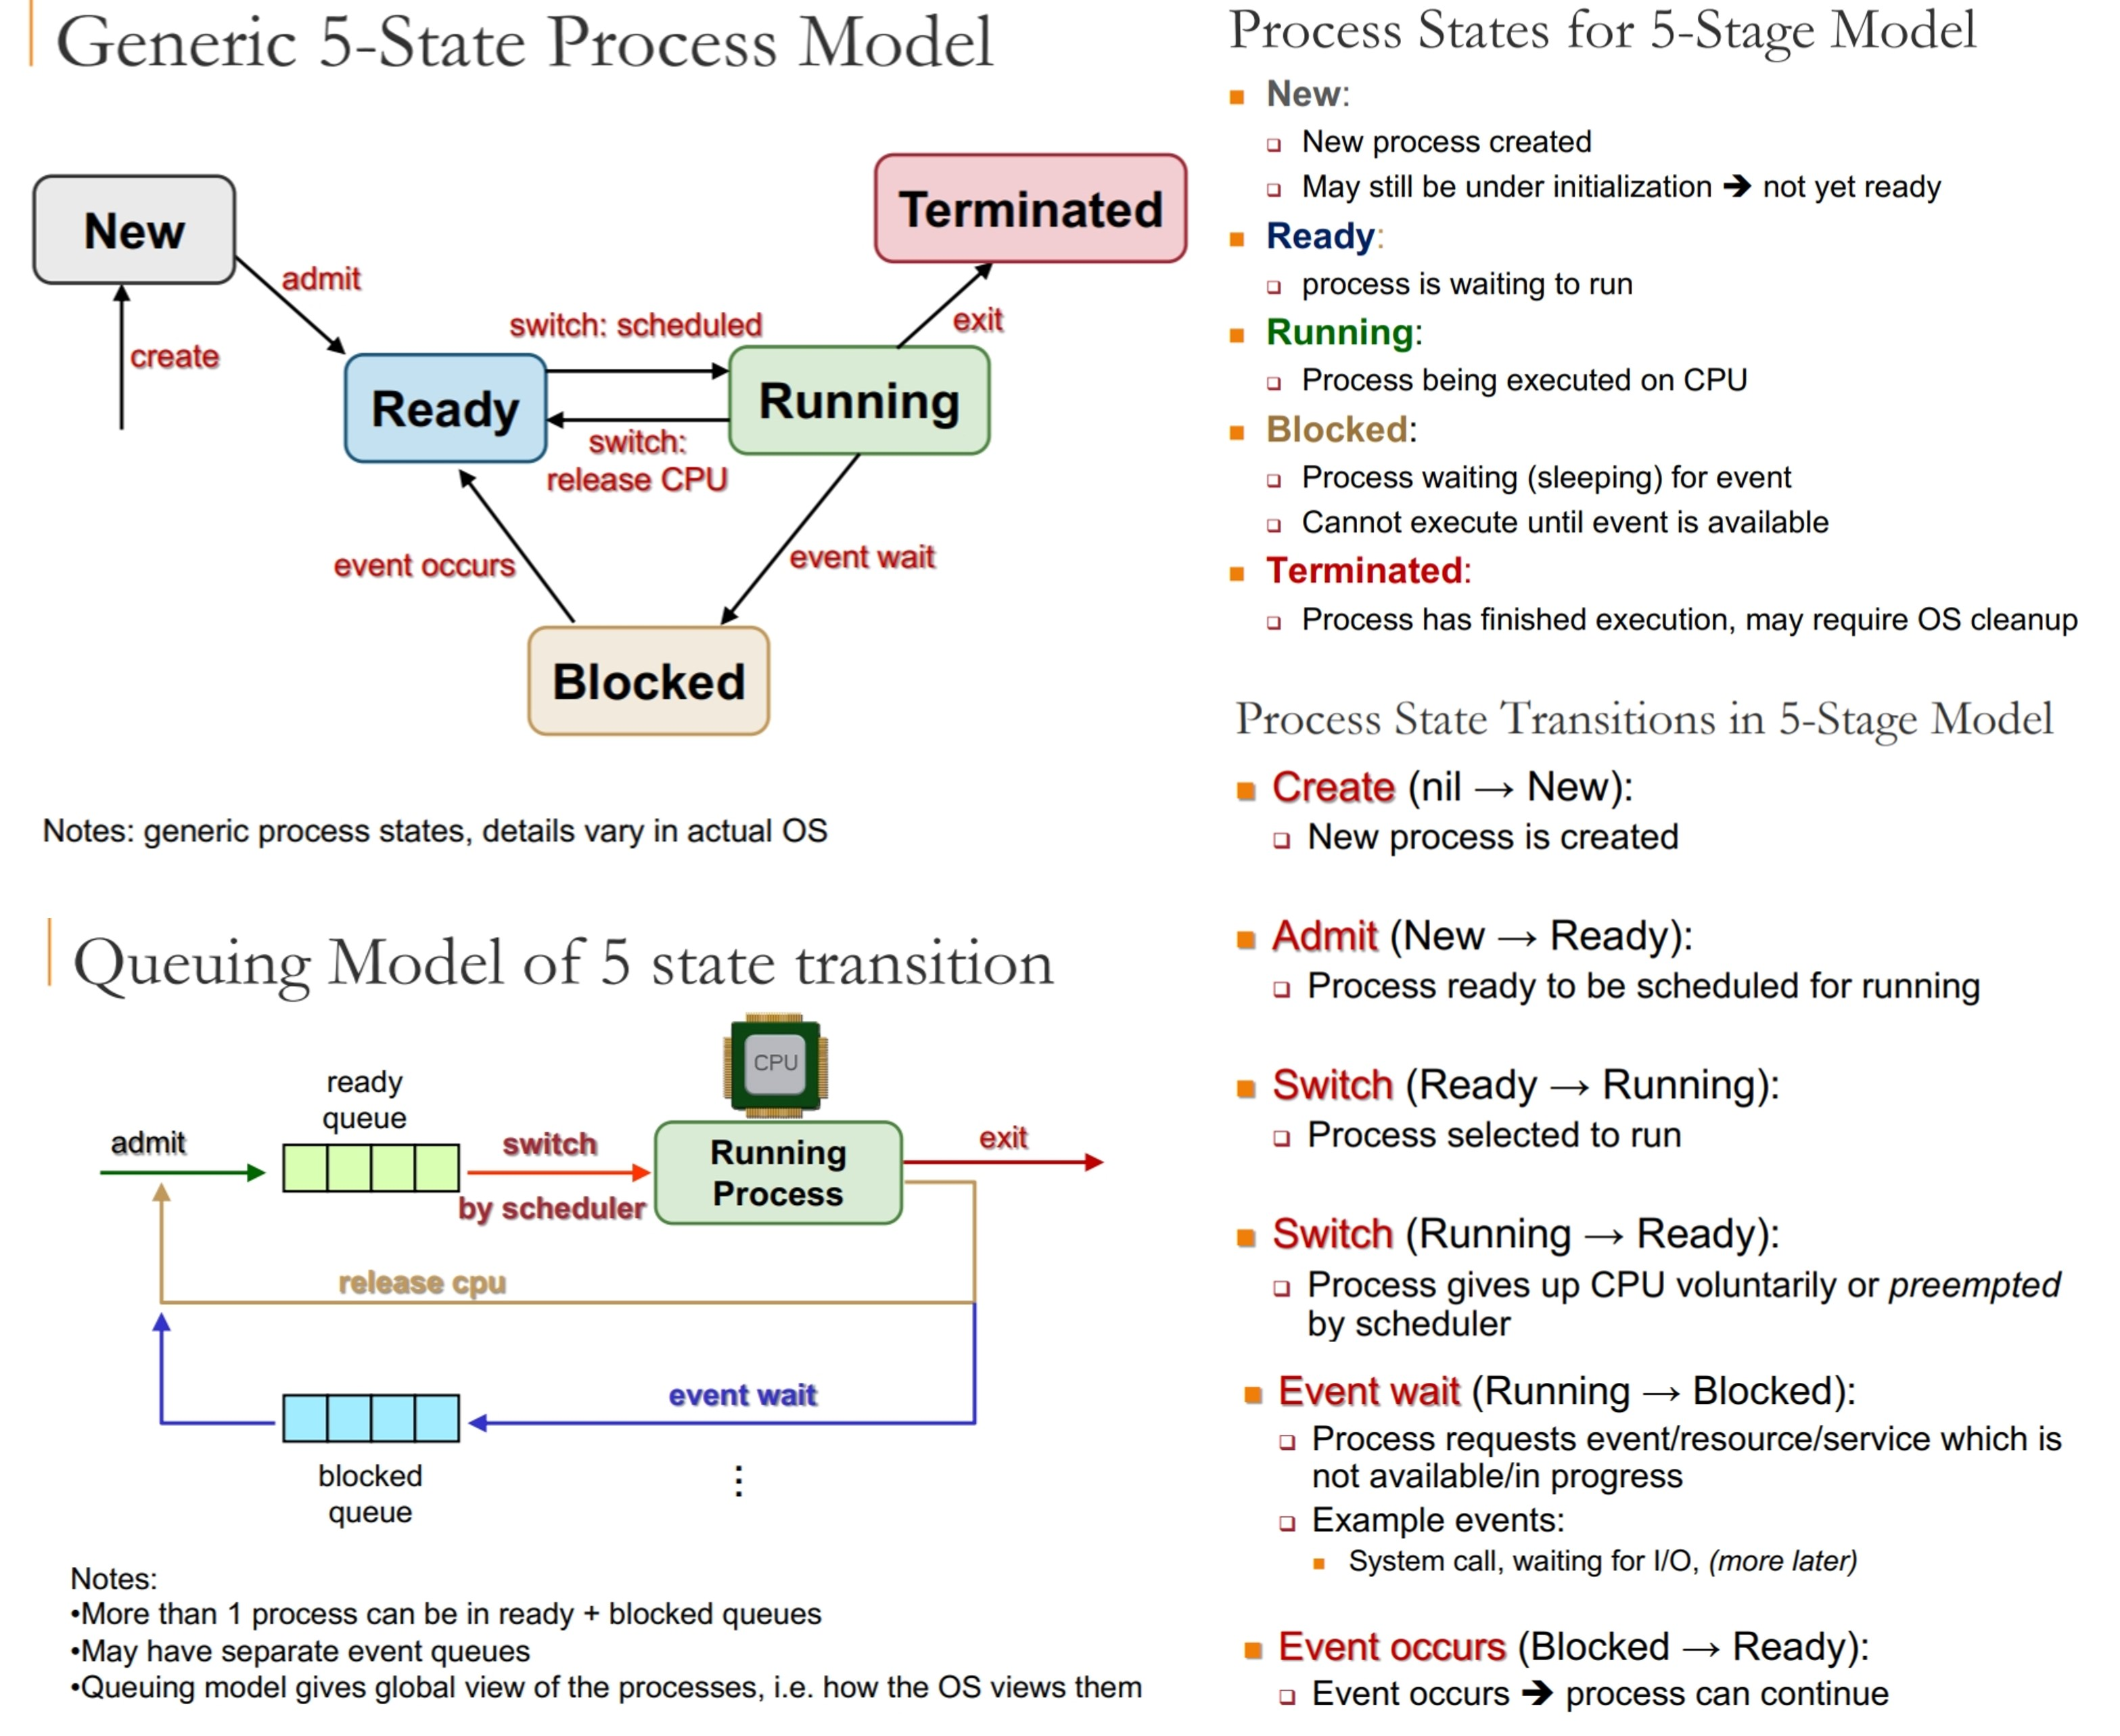
\includegraphics[width=1\linewidth]{5StateProcess}}

\subsection{Process Table \& Process Control Block}
\begin{itemize}
\item Since the OS is just a program as well, need to make use of data structures to track these processes.
\item \textbf{Process Control Block (PCB) or Process Table Entry}: Entire Execution Context for a process.
\item Kernel maintains \textbf{PCB} for all processes. (Conceptually stored as one table representing all processes.)
\item \textbf{Factors to consider}: \\
- Scalability (how many concurrent processes at once). \\
- Efficiency (should provide efficient access with minimum space wastage).
\end{itemize}
\centerline{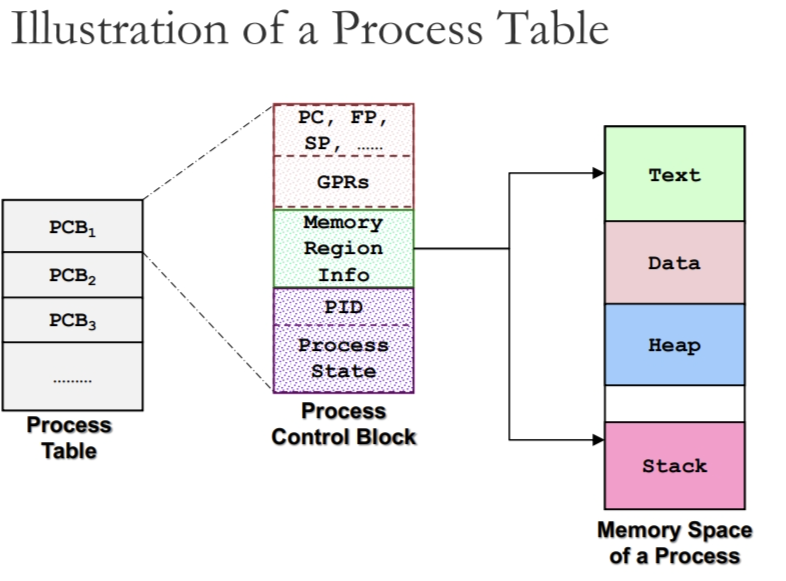
\includegraphics[width=0.6\linewidth]{processTable}}

\subsection{Process Abstraction in Unix}
\begin{itemize}
\item \textbf{Process Identification, Information}
\end{itemize}
\centerline{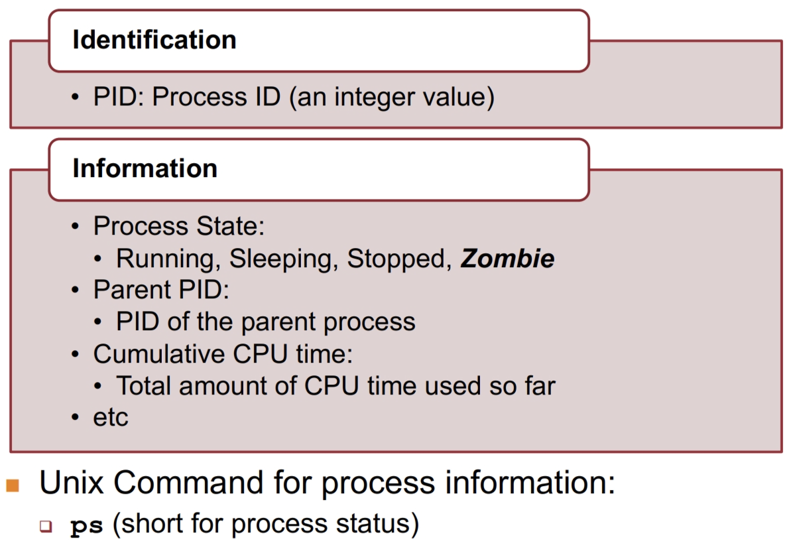
\includegraphics[width=0.6\linewidth]{processAbstraction}}
\begin{itemize}
\item \textbf{Process Creation, Termination, Parent-Child Synchronization}
\end{itemize}

\subsubsection{Note: Command Line Argument in C}
\begin{itemize}
\item We can pass arguments to a program in C.
\item \code{argc}: Number of CL arguments, including program name.
\item \code{argv}: A char strings array, each element in \code{argv[]} is a C character string.
\end{itemize}
\begin{lstlisting} [linewidth = 1.0 \linewidth],
int main( int argc, char* argv[] )
{ int i;
	 for (i = 0; i < argc; i++){
	 printf("Arg \%i: \%s, ",i, argv[i] );
	 }
	 return 0;
}
\end{lstlisting}
\begin{itemize}
\item Example Run: ``a.out 123 hello world''
\item Output: ``Arg 0: a.out, Arg 1: 123, Arg 2: hello, Arg 3: world''
\end{itemize}

\subsubsection{Process Creation: \code{fork()}}
\centerline{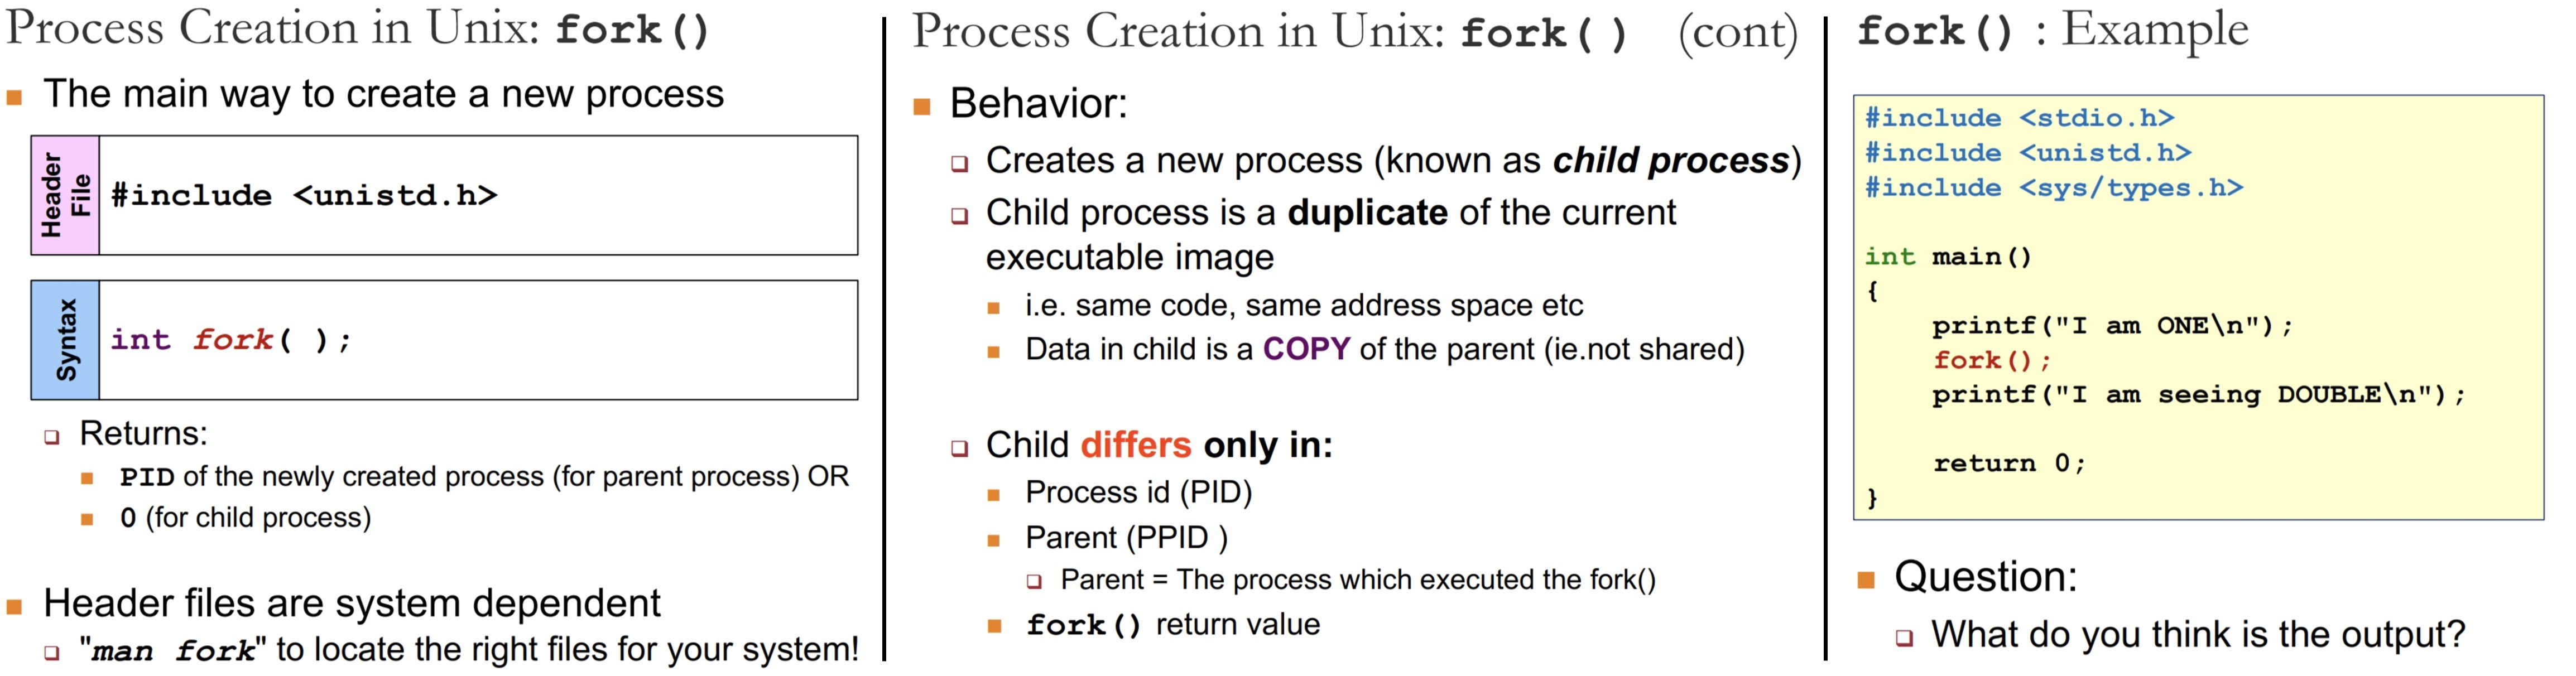
\includegraphics[width=1\linewidth]{processCreation}}
\begin{itemize}
\item \code{fork()}: Create exact copy of the parent, including any variables.
\item \textbf{Output}: Both parent and child resume execution after the point \code{fork()}. 
\item \textbf{Note \code{clone()}}: \code{fork()} not versatile, for scenarios where partial duplication preferred, \code{clone()}, which supersedes \code{fork()}.
\item Both parent and child processes continue executing, common usage is to use the parent/child process differently. (Parent spawn off child to carry out some work, parent ready to take another order.) \\
- Use return value of \code{fork()} to distinguish parent and child.
\end{itemize}
\centerline{\includegraphics[width=0.4\linewidth]{forkResult}}


\subsubsection{Process Replacement: \code{execl()} System Call}
\begin{itemize}
\item Function \textbf{replaces current executing process image} with a new process image specified by path. No return is made because the calling process image is replaced by the new process image.
\item \textbf{Code Replacement}, but \textbf{PID and other information still intact}.
\end{itemize}
\centerline{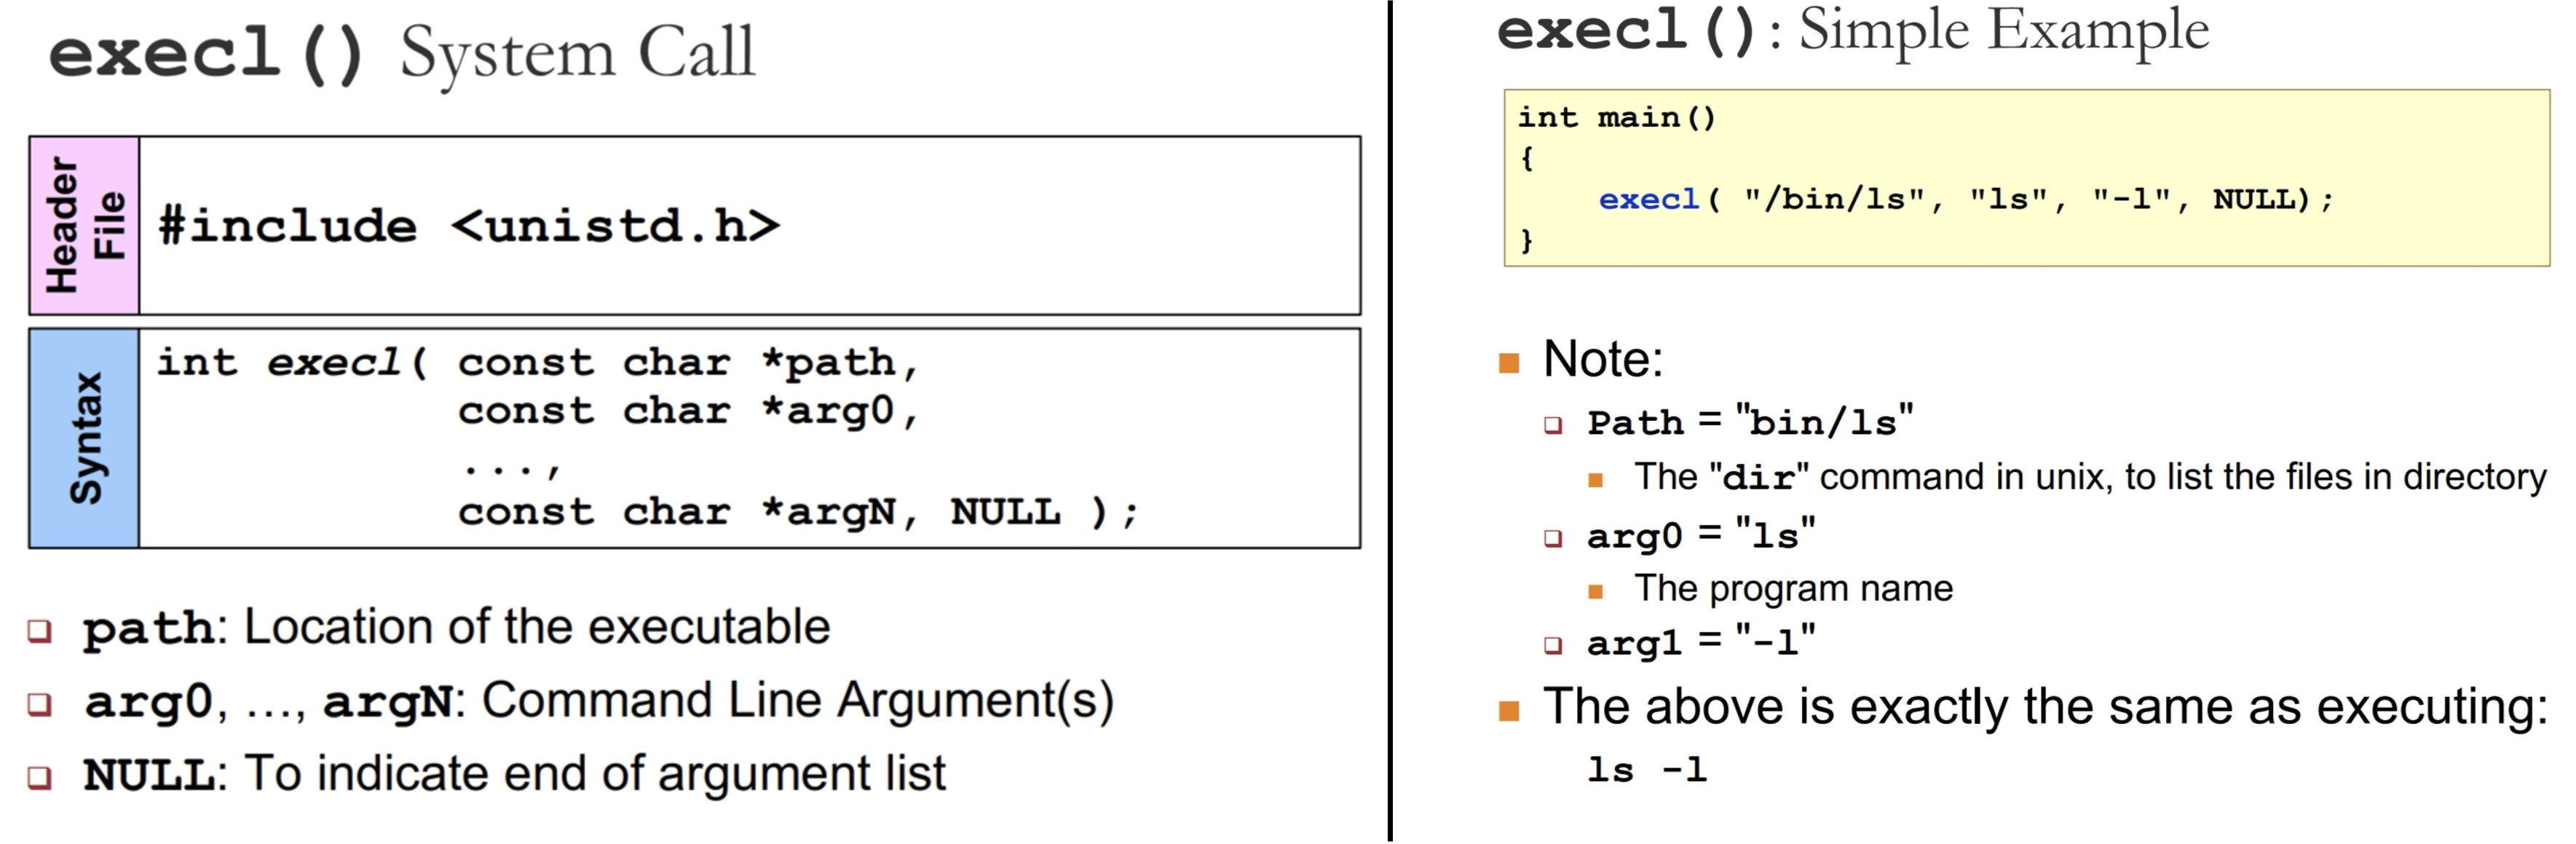
\includegraphics[width=0.95\linewidth]{execl}}
\begin{itemize}
\item \textbf{By combining \code{fork()} and \code{exec()}}, we can spawn off a child process (let it perform task through \code{exec()}), while parent process around to accept another request.
\item This combination of mechanisms is main way in Unix to get new process for running new program!
\end{itemize}

\subsection{The Master Process: \code{init}}
\begin{itemize}
\item Every process has parent process, consider special initial process.
\item \textbf{\code{init} process}: Created in kernel at boot up time, usually PID = 1. 
\item \textbf{Purpose}: Watches and respawns other (critical) processes where needed.
\item \code{fork()} creates the process tree, where \code{init} is the root process.
\end{itemize}

\subsubsection{Simplified Process Tree Ex.}
\centerline{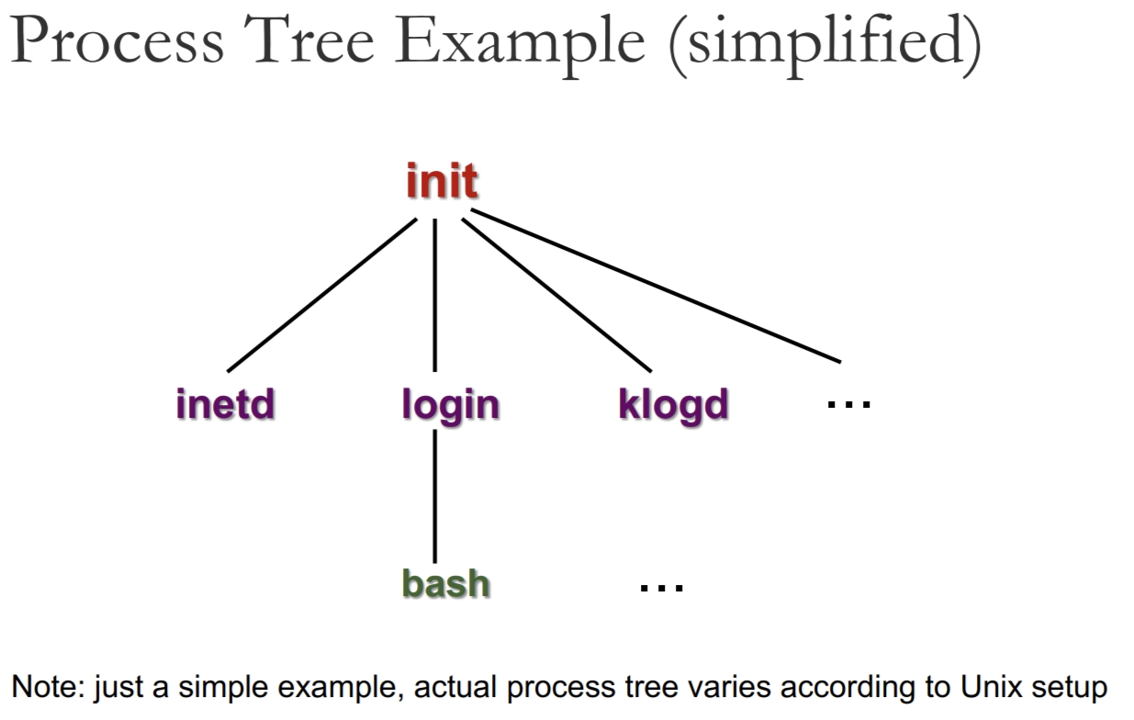
\includegraphics[width=0.6\linewidth]{processTree}}
\begin{itemize}
\item \textbf{d}, (e.g. \code{klogd}) at end of process name usually means server process (Daemon, background process.)
\end{itemize}

\subsubsection{Process Termination in Unix: \code{exit}}
\centerline{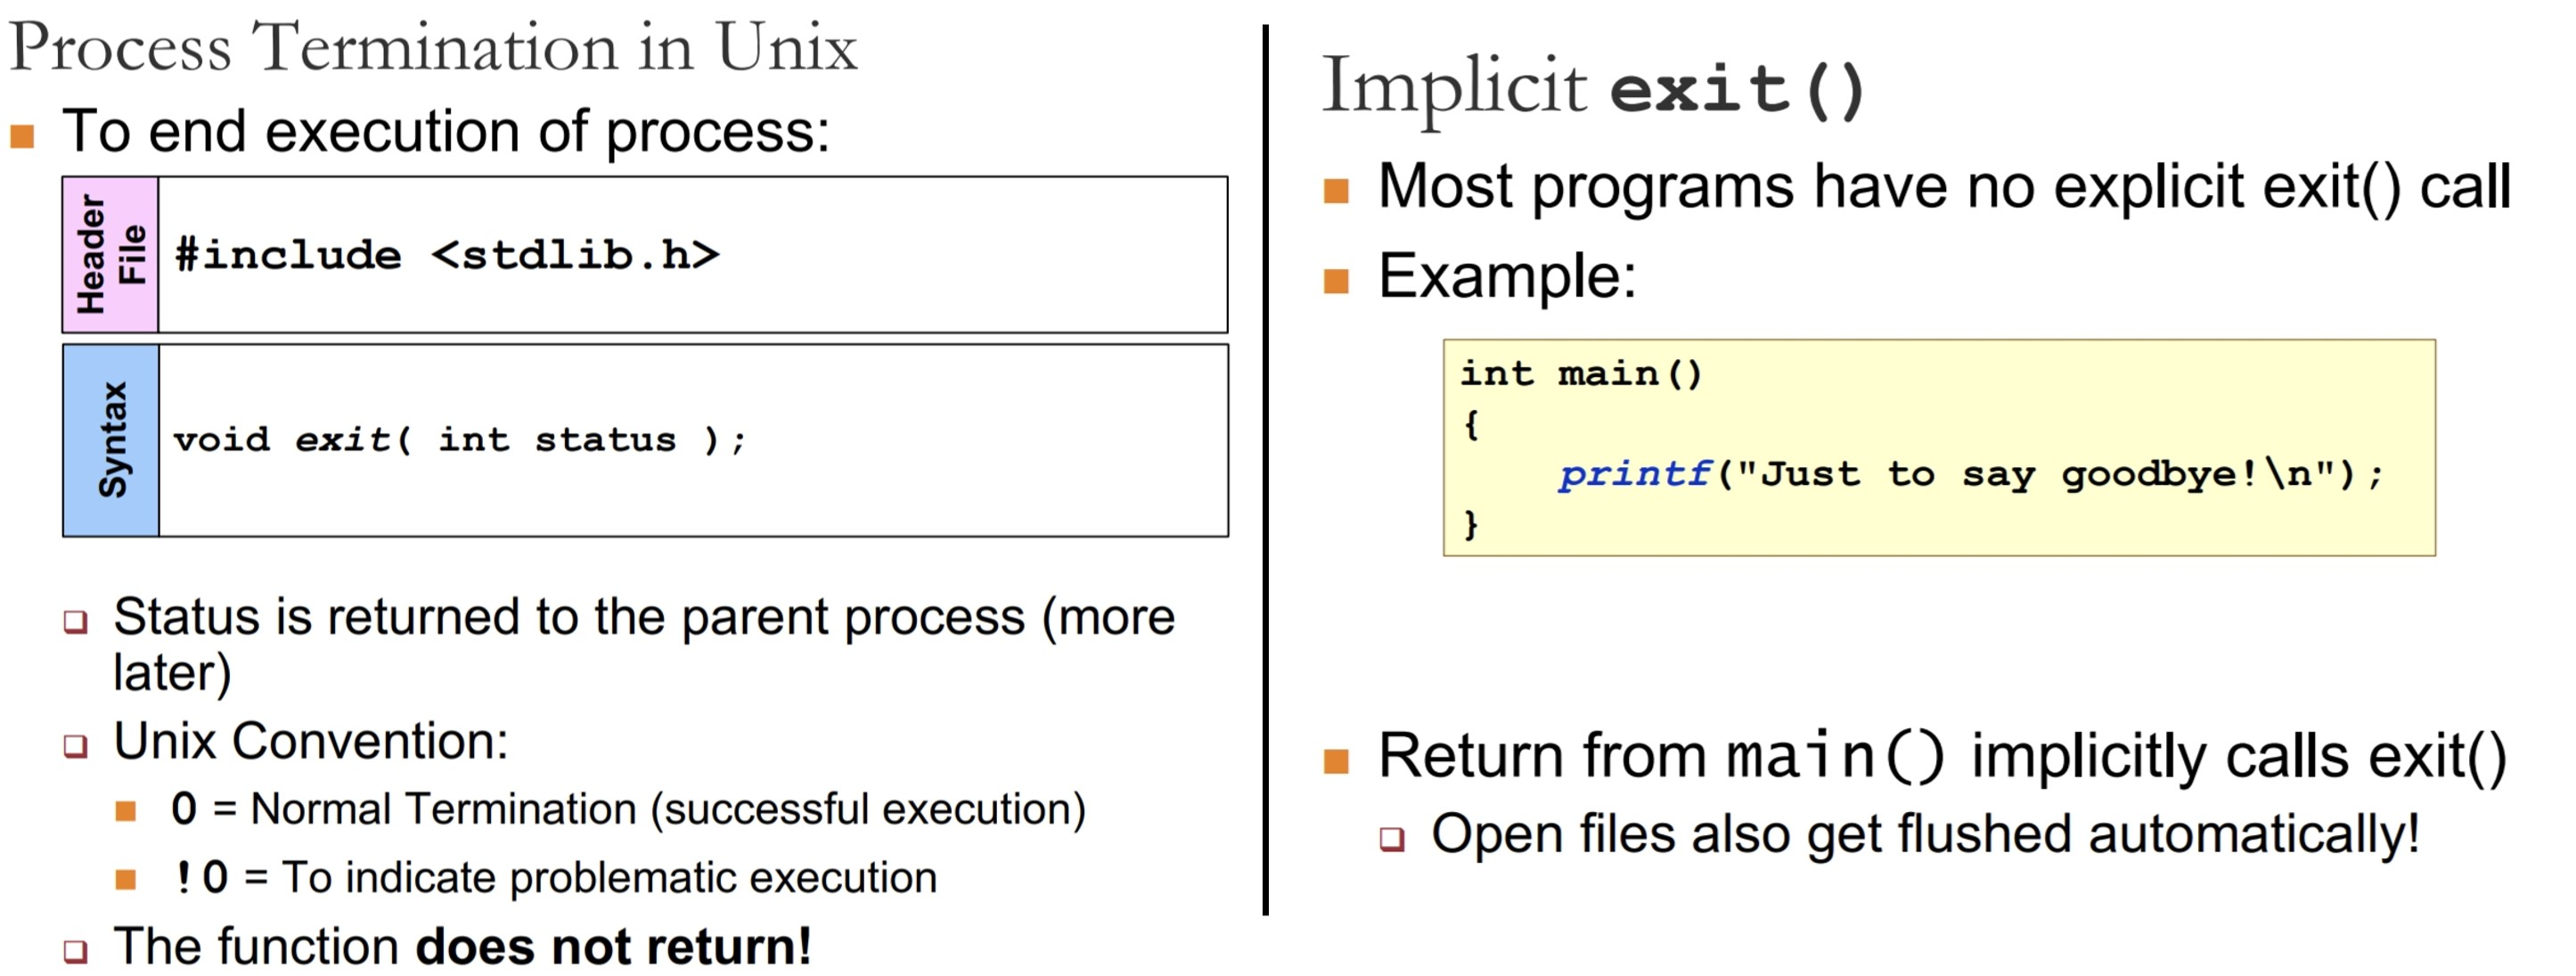
\includegraphics[width=1\linewidth]{processTermination}}
\medskip
\begin{itemize}
\item \textbf{Process finished execution}: \textbf{Most} system resources used by process are released on exit. (e.g. file descriptors).
\item \textbf{Certain basic process resources not Releasable}: PID, status needed. For parent-children synchronization, for parent to check status of child, For process accounting info (e.g. cpu time).
\item Process table entry may still be needed after termination.
\end{itemize}

\subsubsection{Parent/Child Synchronization in Unix}
\begin{itemize}
\item Parent process can wait for child process to terminate.
\item Argument is a pointer to a variable that will store the return value (\code{*status}).
\end{itemize}
\centerline{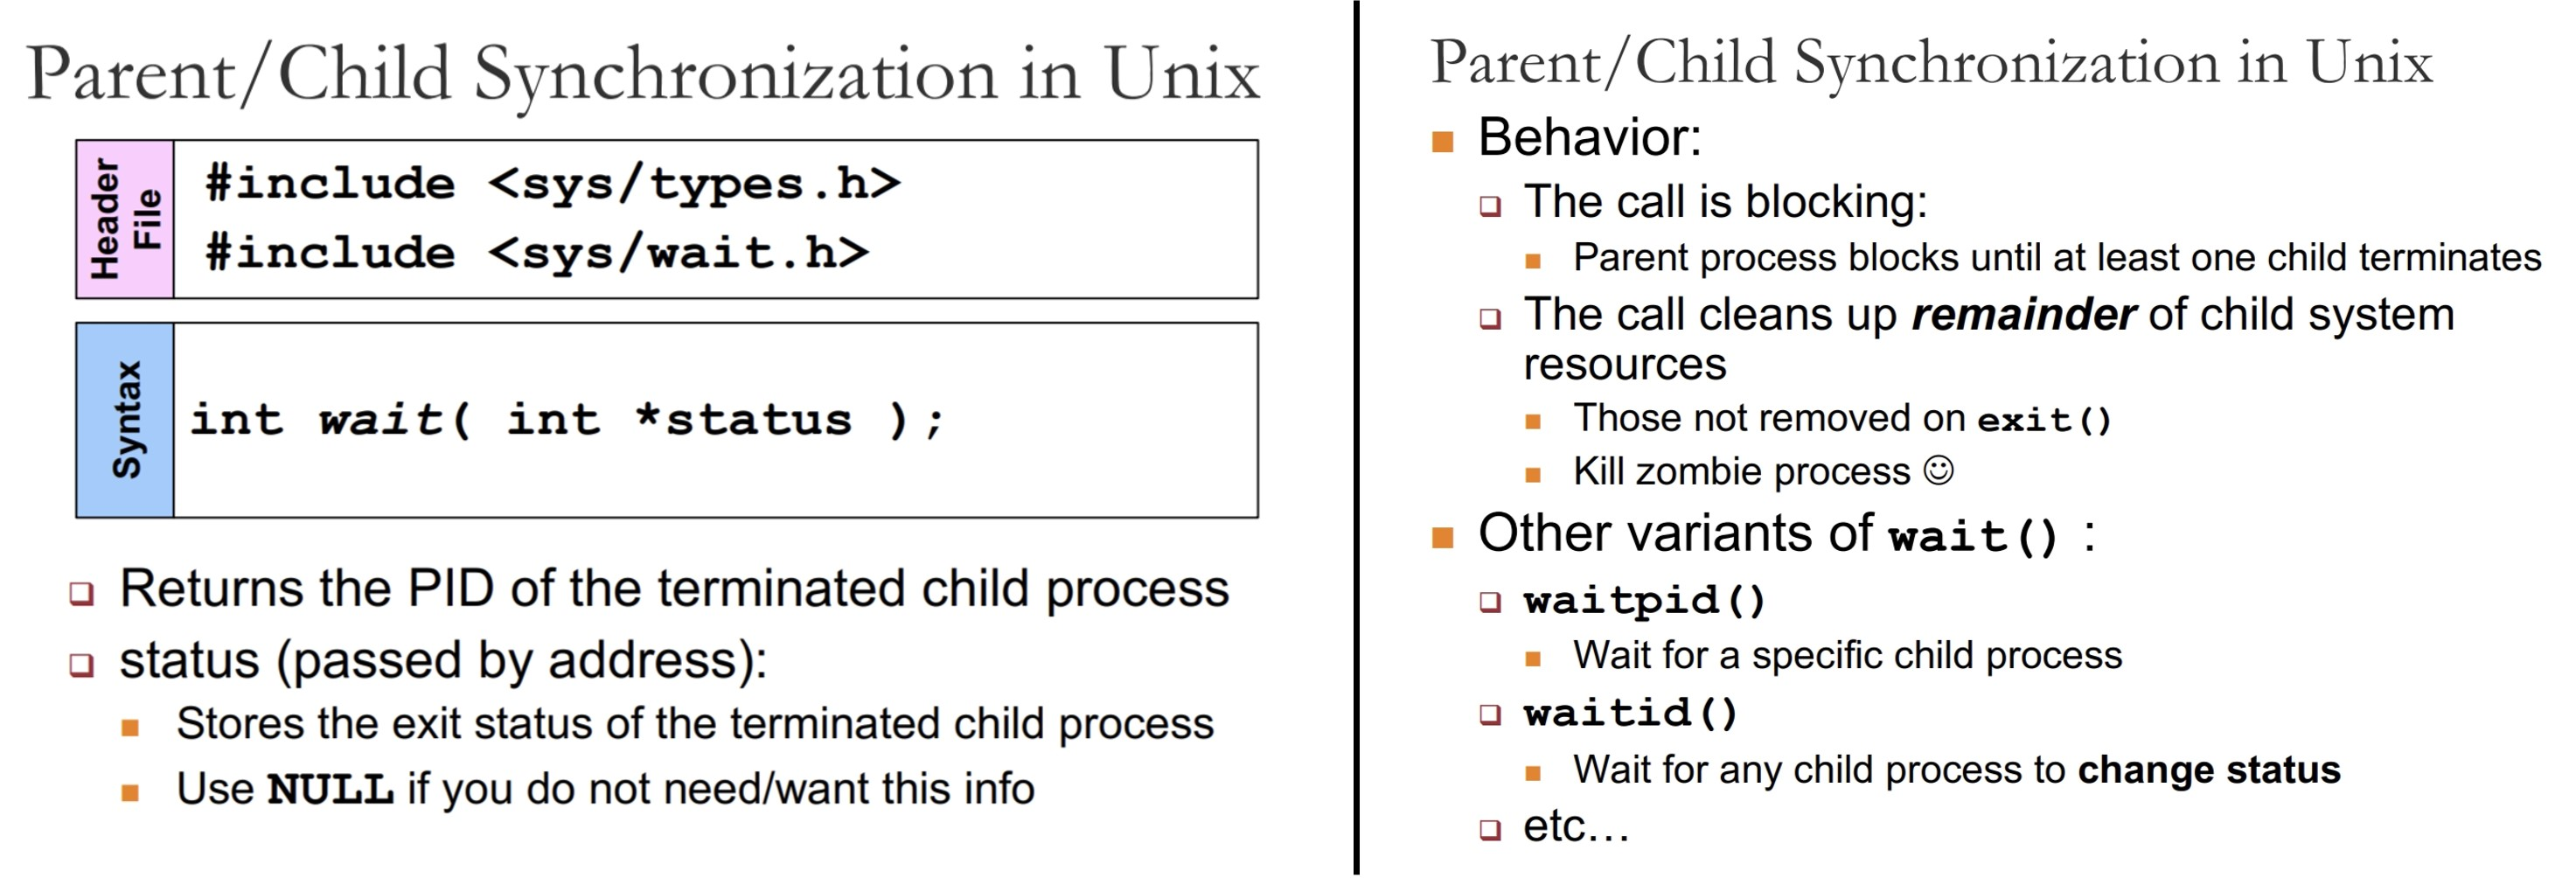
\includegraphics[width=1\linewidth]{PCSynchronization}}
\begin{itemize}
\item Kills zombine processes! With enough zombies, process table finite size, run out of space.
\end{itemize}
\centerline{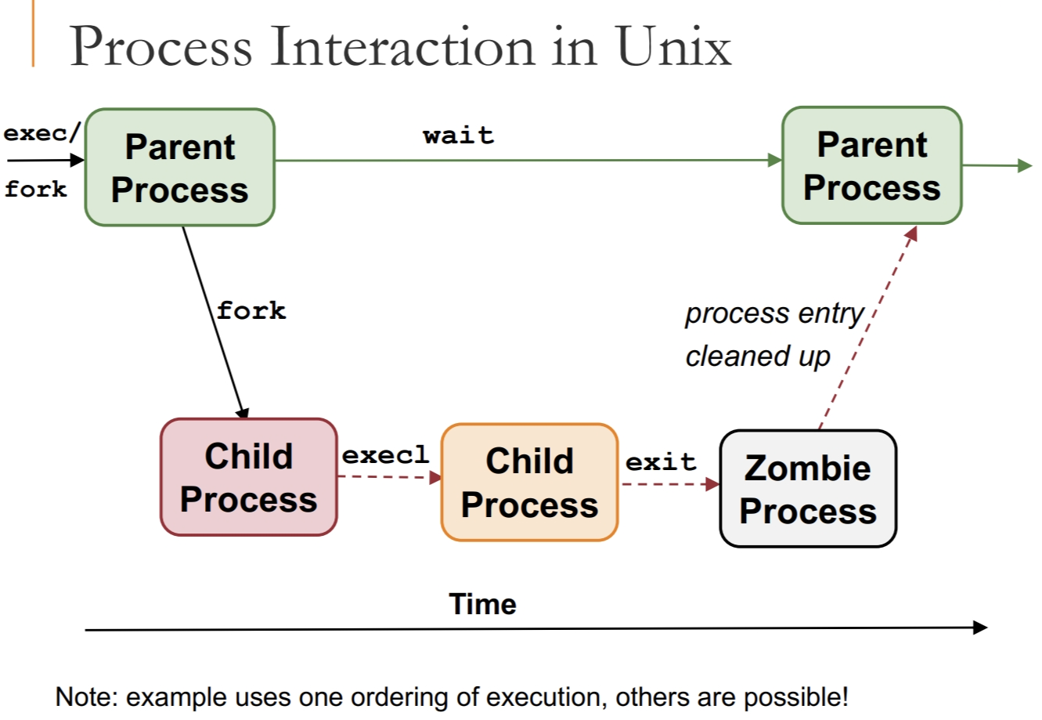
\includegraphics[width=0.5\linewidth]{processInteraction}}

\subsubsection{Zombie Processes (2 Cases)}
\begin{itemize}
\item \code{wait()} ``creates'' the zombies (and later cleans it up) as on process exit, process becomes zombie.
\item Since it cannot delete all process info (if parent asks for info in \code{wait()} call, remainder of process data structure can be cleaned up only when \code{wait()} happens.)
\item We cannot \code{kill PID} zombie process, is already dead. Until restart system or modern OS look through table and remove them.
\end{itemize}

\begin{enumerate}
\item \textbf{Parent process terminates before child process}
	\begin{itemize}
	\item \code{init} process becomes "pseudo" parent of child processes.
	\item Child termination sends signal to \code{init}, which utilizes \code{wait()} to cleanup 
	\end{itemize}
\item \textbf{Child process terminates before parent but parent did not call wait}
	\begin{itemize}
	\item Child process become a zombie process
	\item Can fill up / hog process table, May need a reboot to clear the table on older Unix implementations
	\end{itemize}
\end{enumerate}
\centerline{\includegraphics[width=1\linewidth]{processSummary}}

\section{Implementation Issues}
\subsection{Implementing \code{fork()}}
\centerline{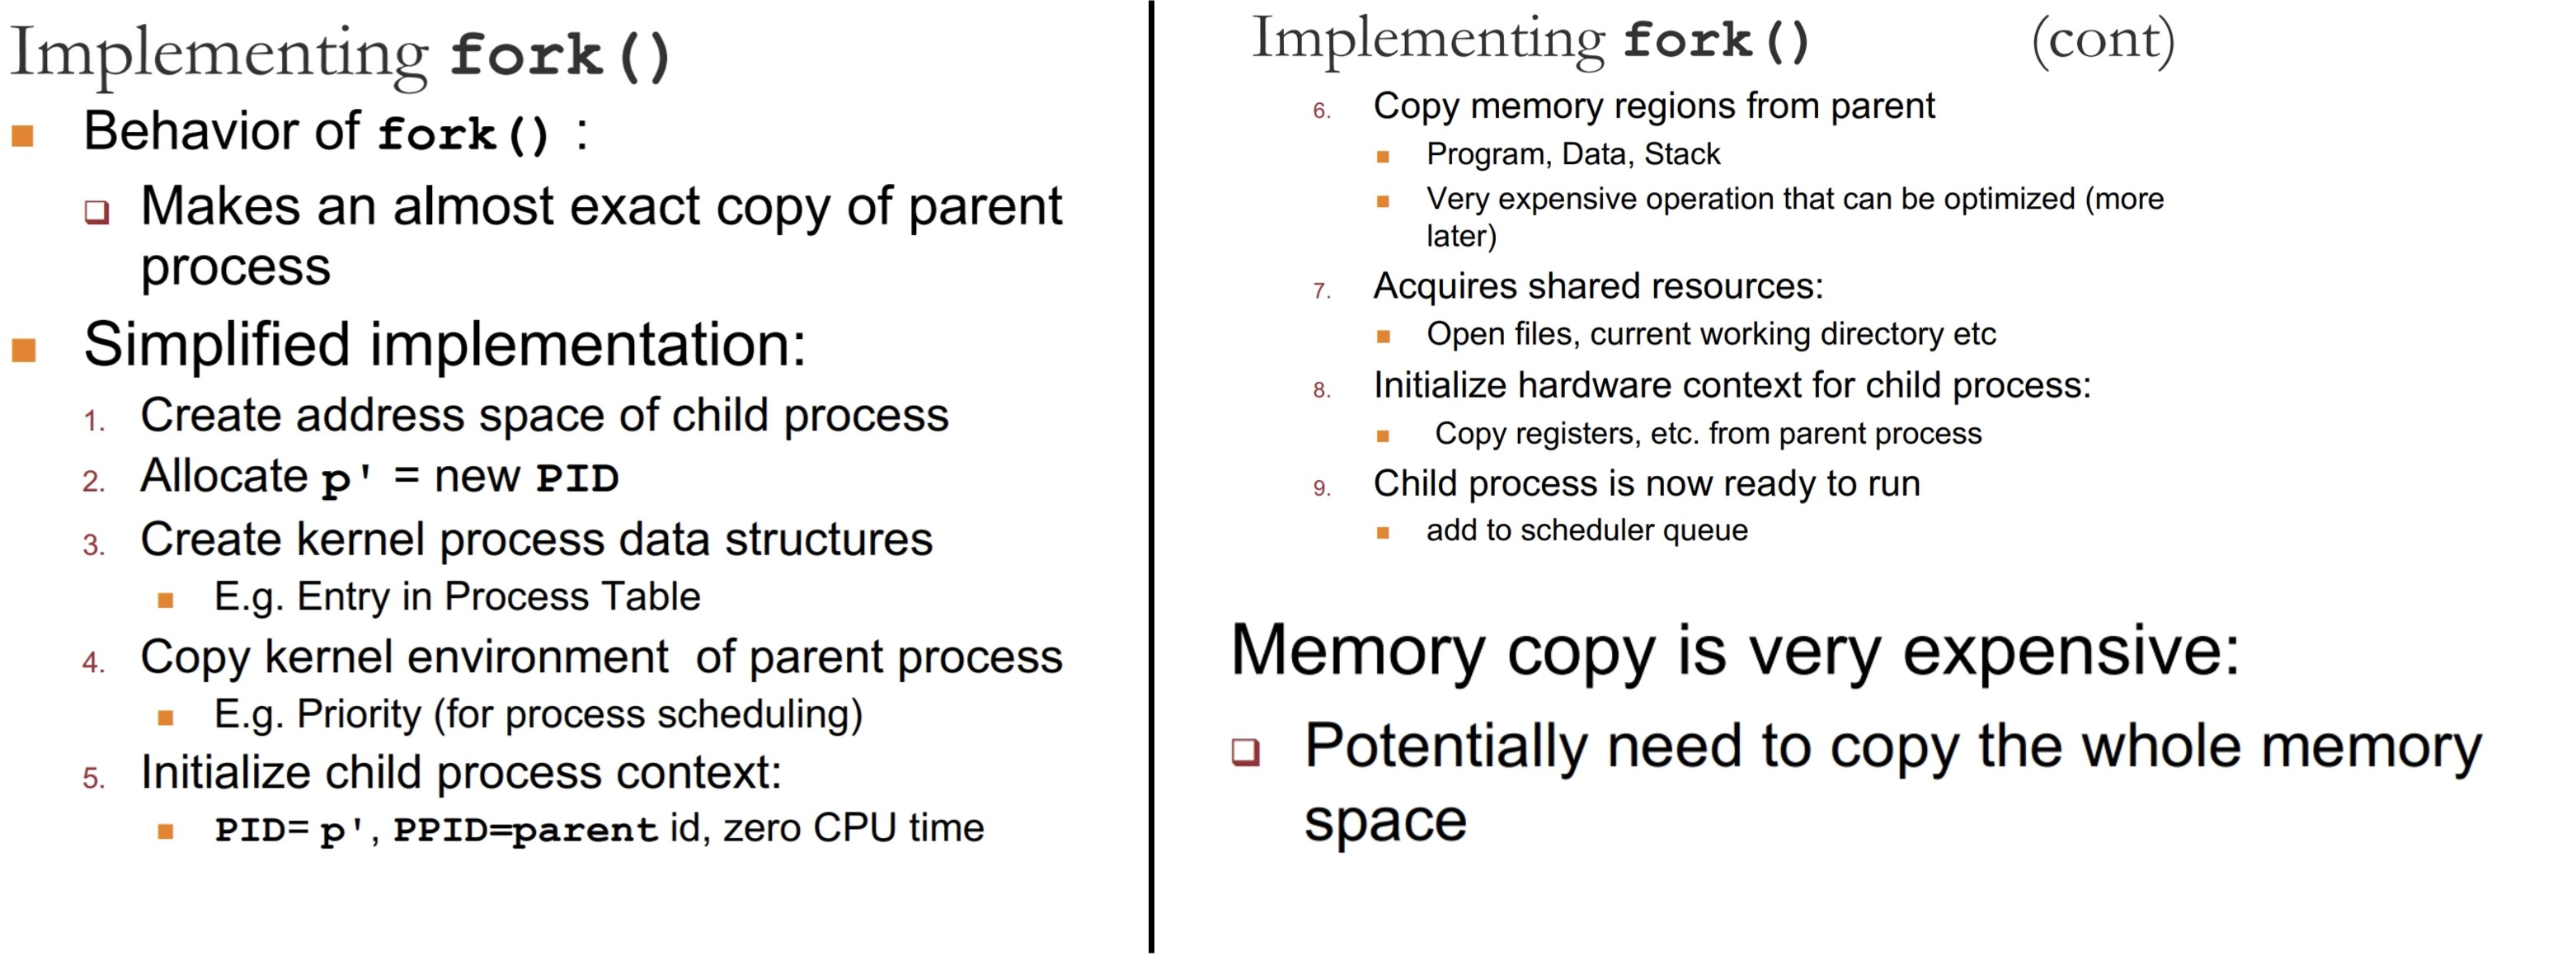
\includegraphics[width=0.95\linewidth]{implementFork}}
\begin{itemize}
\item \textbf{Copying entire memory space is wasteful} and not always needed! (E.g. copy entire 200mb program image of Zoom etc). Mostly, only need contents, and PC, register values.
\item \textbf{Give Rise to COW.} (copy on write)
\end{itemize}

\subsection{Memory Copy Operation}
\begin{itemize}
\item If child just read from location, unchanged, just use a shared version.
\item \textbf{Only when write is perform on a location, then two independent copies needed.}
\item \textbf{Copy on Write} is possible optimization, only duplicate ``memory location'' when it is written to, otherwise parent and child share same ``memory location''.
\item Note: memory organized into memory pages (consec range of mem locations), memory managed on page level instead of individual location.
\end{itemize}

\section{System Calls (Process Interaction with OS)}
\subsection{API to OS: Application Program Interface to OS}
\begin{itemize}
\item OS API provides way of calling facilities/services in kernel.
\item \textbf{Not same as normal function call}: Change from \textit{user mode to kernel mode}.
\item Different OS have different APIs: Unix Variants most follow POSIX standards, small no. of calls ~100. Windows family uses Win API across diff. windows, huge no. of calls ~1000.
\end{itemize}

\subsection{Unix System Calls in C/C++ program}
\begin{itemize}
\item In C/C++ program, \textbf{system call can be invoked almost directly}, as library version very closely reflects these calls.
\item Majority of system calls have library version with \textbf{same name} and parameters, library version acts as \textbf{function wrapper}. 
\item A few library functions present more user friendly version, e.g. less no. /more flexible parameters). Library version acts as \textbf{function adapter}.
\end{itemize}
\centerline{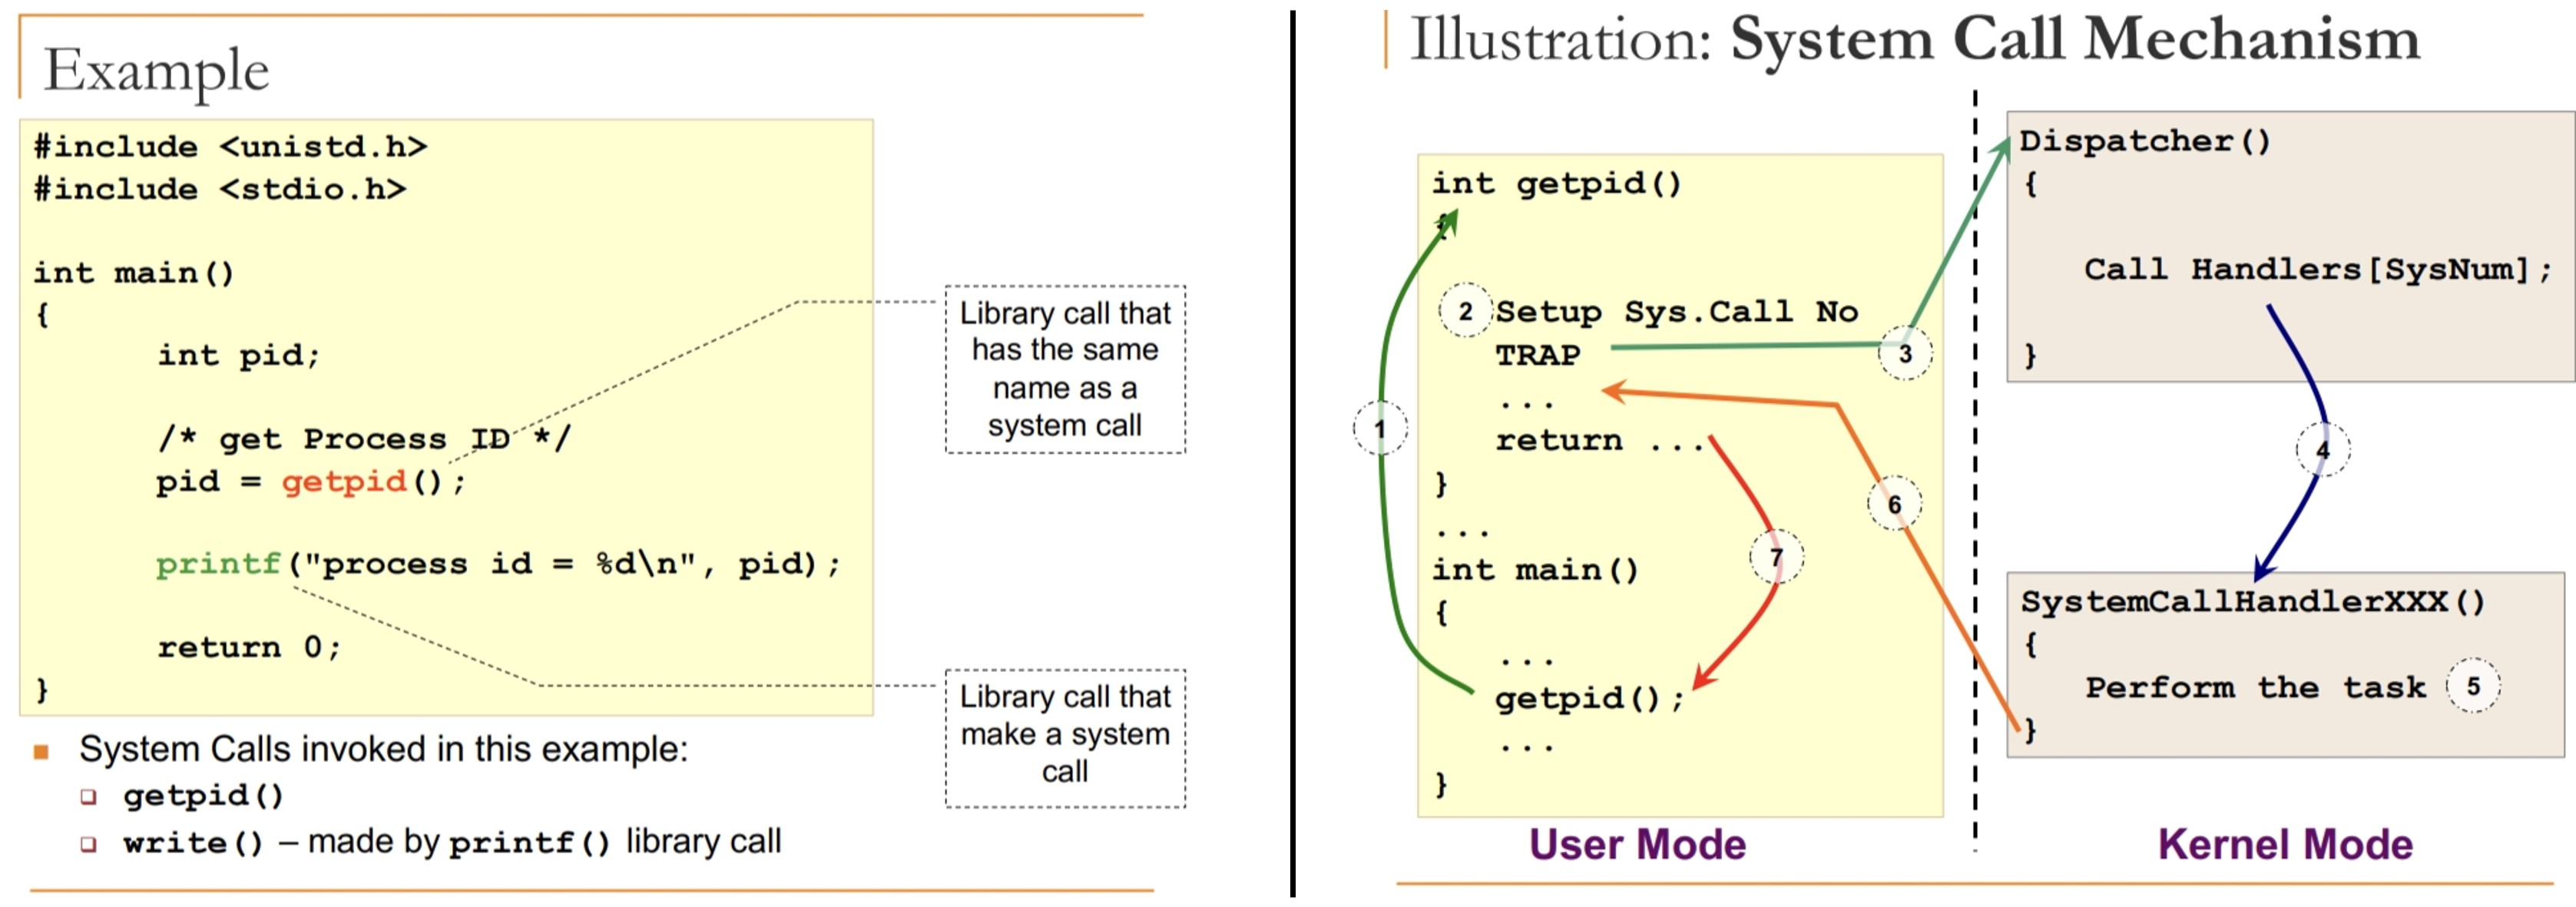
\includegraphics[width=1\linewidth]{systemCallExample}}

\subsection{General System Call Mechanism}
\centerline{\includegraphics[width=1\linewidth]{generalSystemCallMechanism}}

\section{Exception and Interrupt}

\subsubsection{Exception}
\begin{itemize}
\item \textbf{Executing machine level instruction} can cause \textbf{exception}. For example:
\begin{itemize}
\item Airthmetic Errors: Overflow, Underflow, Division by Zero
\item Memory Accessing Errors: (accessing memory not belonging to program), Illegal memory address, mis-aligned memory access.
\end{itemize}
\item Exception is \textbf{Synchronous}: Determinate, occurs due to program execution at exact points of time.
\item \textbf{Effect of Exception}: Have to execute \textbf{exception handler}, which is similar to a \textbf{``forced function call''!}
\item Exception $\neq$ Interrupt!
\end{itemize}

\columnbreak

\subsubsection{Interrupt}
\begin{itemize}
\item \textbf{External events} can interrupt the execution of a program.
\item Interrupt request lines connected to CPU, lines are checked during instruction execution cycle.
\item Usually hardware related, e.g.: Timer, Mouse move, Keyboard press etc
\item Interrupt is \textbf{asynchronous}: Events occurs independent of program execution.
\item \textbf{Effect of interrupt:} Program execution, suspended, execute an interrupt handler.
\end{itemize}
\centerline{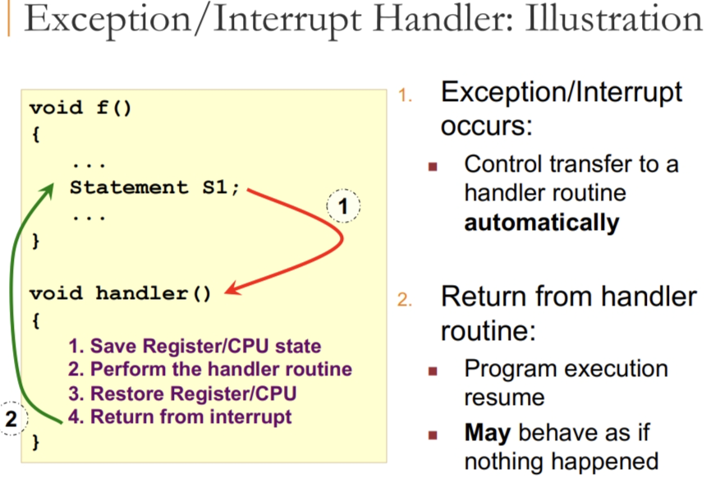
\includegraphics[width=0.5\linewidth]{ExceptionHandler}}

\subsection{Summary}
\begin{itemize}
\item Using \textbf{process as an abstraction} of running program.
\item Includes necessary information (environment) of execution, Memory, Hardware and OS contexts.
\item \textbf{Process from OS perspective}: PCB and process table
\item \textbf{How OS \& Process interact}: System calls, Exception / Interrupt
\end{itemize}

\subsubsection{REFER TO TEXTBOOK:}
\begin{itemize}
\item Modern Operating System (3rd Edition): Section 2.1
\item Operating System Concepts (8th Edition): Section 3.1
\end{itemize}

\vfill \null
\columnbreak

\section{3. Process Scheduling}
A multiprogrammed computer frequently has multiple processes/threads computing for CPU at the same time. Occurs whenever $\geq$ 2 simultaneously in ready state. 
\begin{itemize}
\item \textbf{Scheduler}: Part of OS to decide which process to run next.
\item \textbf{Scheduling Algorithm}: Algo used.
\item \textbf{Scheduling Problem}: Choosing, ready process $>$ available CPUs.
\item In addition to picking right process, need \textbf{efficient use of CPU} as process switching is expensive. (Switch user to kernel mode, save state of process, memory map, memory cache may need to reload, etc.)
\item \textbf{I/O Input/Output} (disk or network): When process enters blocked state waiting for external device to complete work.
\end{itemize}

\subsubsection{Process Behavior}
\begin{itemize}
\item Process' unique \textbf{requirement of CPU time.}
\item Process goes through phases of CPU-activity \& IO-activity.
\item \textbf{Compute/CPU-Bound Process} (computation, e.g. number crunching) vs. \textbf{IO-bound Process} (e.g. read/write to file, print to screen)
\end{itemize}
\centerline{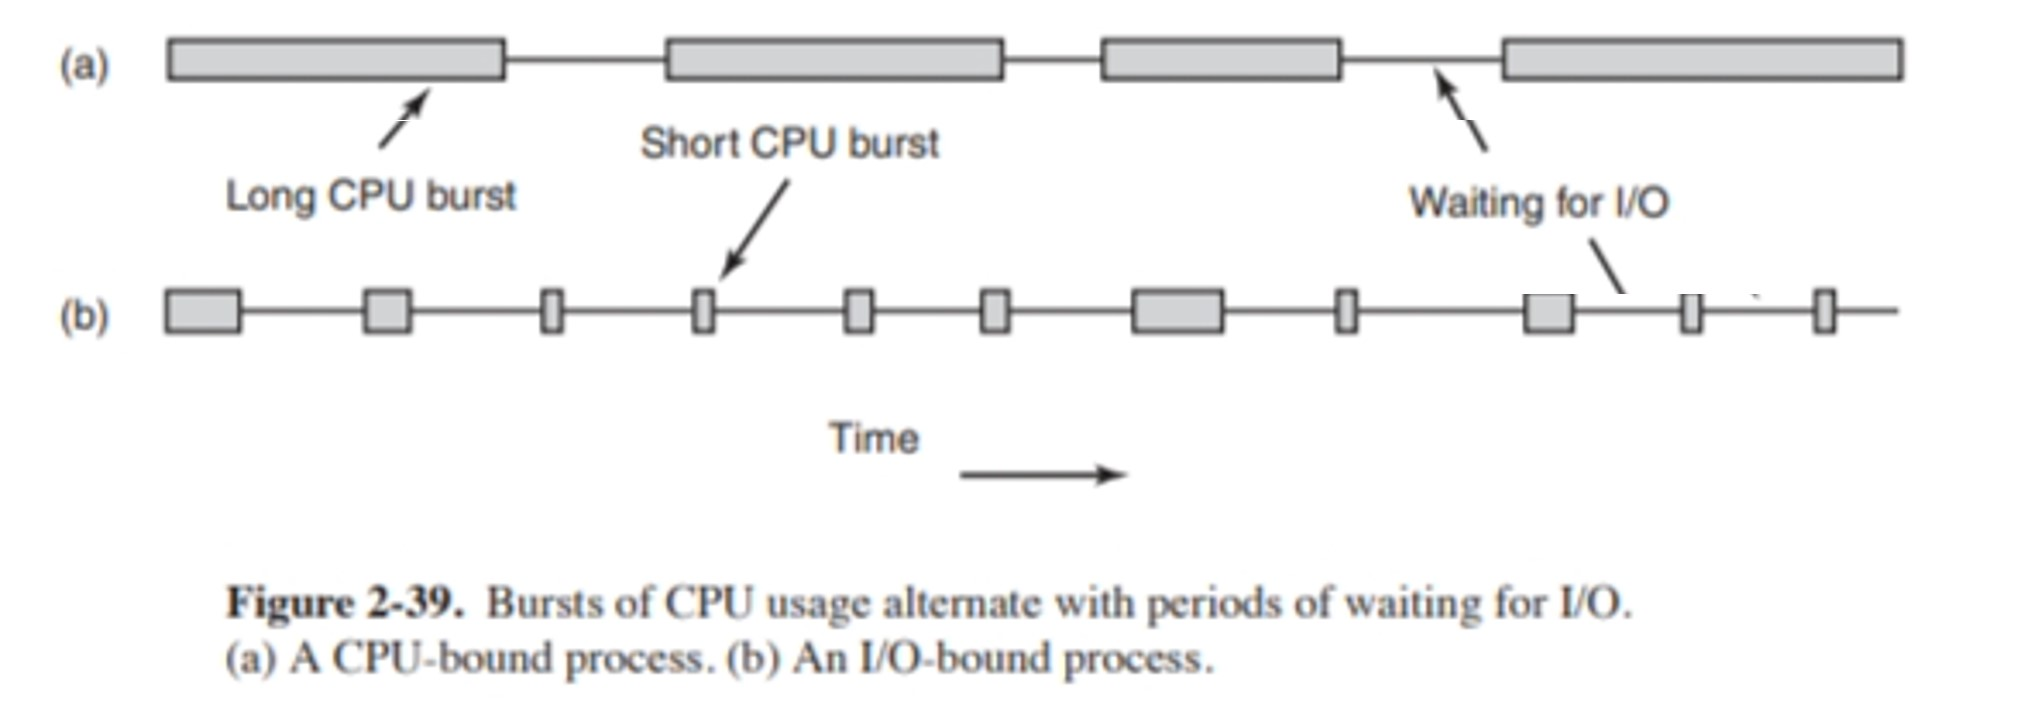
\includegraphics[width=0.7\linewidth]{processBehavior}}

\subsubsection{Process Environment}
\begin{itemize}
\item \textbf{Batch Processing}: No user, no interaction / responsiveness required.
\item \textbf{Interactive / Multiprogramming}: Active user interacting with system. Need responsive, consistent in response time.
\item \textbf{Real Time Processing}: Deadline to meet, usually periodic process.
\end{itemize}

\subsection{Scheduler Evaluation Criteria}
\begin{itemize}
\item Many criteria to evaluating algo, largely influenced by p. environment. May be conflicting.
\item \textbf{All Systems}: \\
- \textit{Fairness}: CPU time (per process basis / per user basis). \textbf{No starvation}. \\
- \textit{Balance}: All parts of computing system utilized.
\item \textbf{Batch Systems}: \\
- \textit{Throughput}: Maximize jobs per hour. \\
- \textit{Turnaround time}: Minimize time btwn. submission \& termination. \\ 
- \textit{++(Waiting Time)}: Related to turnaround, time waiting for CPU \\
- \textit{CPU utilization}: keep CPU busy all the time.
\item \textbf{Interactive Systems}: \\
- \textit{Response time}: respond to requests quickly. \\
- \textit{Proportionality}: meet users' expectations.
\item \textbf{Real-time Systems}: \\
- \textit{Meeting deadlines}: avoid losing data. (e.g. livestream)\\
- \textit{Predictability}: avoid quality degradation in multimedia.
\end{itemize}

\subsection{Concurrent Execution}
\begin{itemize}
\item \textbf{Concurrent Processes}: Logical concept to cover multitasked processes.
\item \textbf{Virtual parallelism}: Illusion of parallelism (pseudo-parallelism)
\item \textbf{Physical parallelism}: Multiple CPUs/Cores, multiple parallel exec
\end{itemize}


\columnbreak

\subsection{When to Schedule}
Key issue, when to make schedule decisions. \\
E.g. When new process created, run parent or child. When process exits, when process blocks on I/O, or I/O interrupt.
\begin{itemize}
\item \textbf{Non-preemptive (cooperative)}: Process stays scheduled (running state) until it blocks, or gives up CPU voluntarily.
\item \textbf{Preemptive (Fixed Quota)}: Process given fixed time quota to run (possible to block / give up early). At end of quota, running process suspended, another picked if available.
\end{itemize}


\subsubsection{Interleaved Execution (Timeslicing)}
\begin{itemize}
\item \textbf{Concurrent Execution on 1 CPU}: Interleave instructions from both processes.
\item \textbf{OS overhead}: Multitasking needs to change context between programs, incurs overhead.
\end{itemize}
\centerline{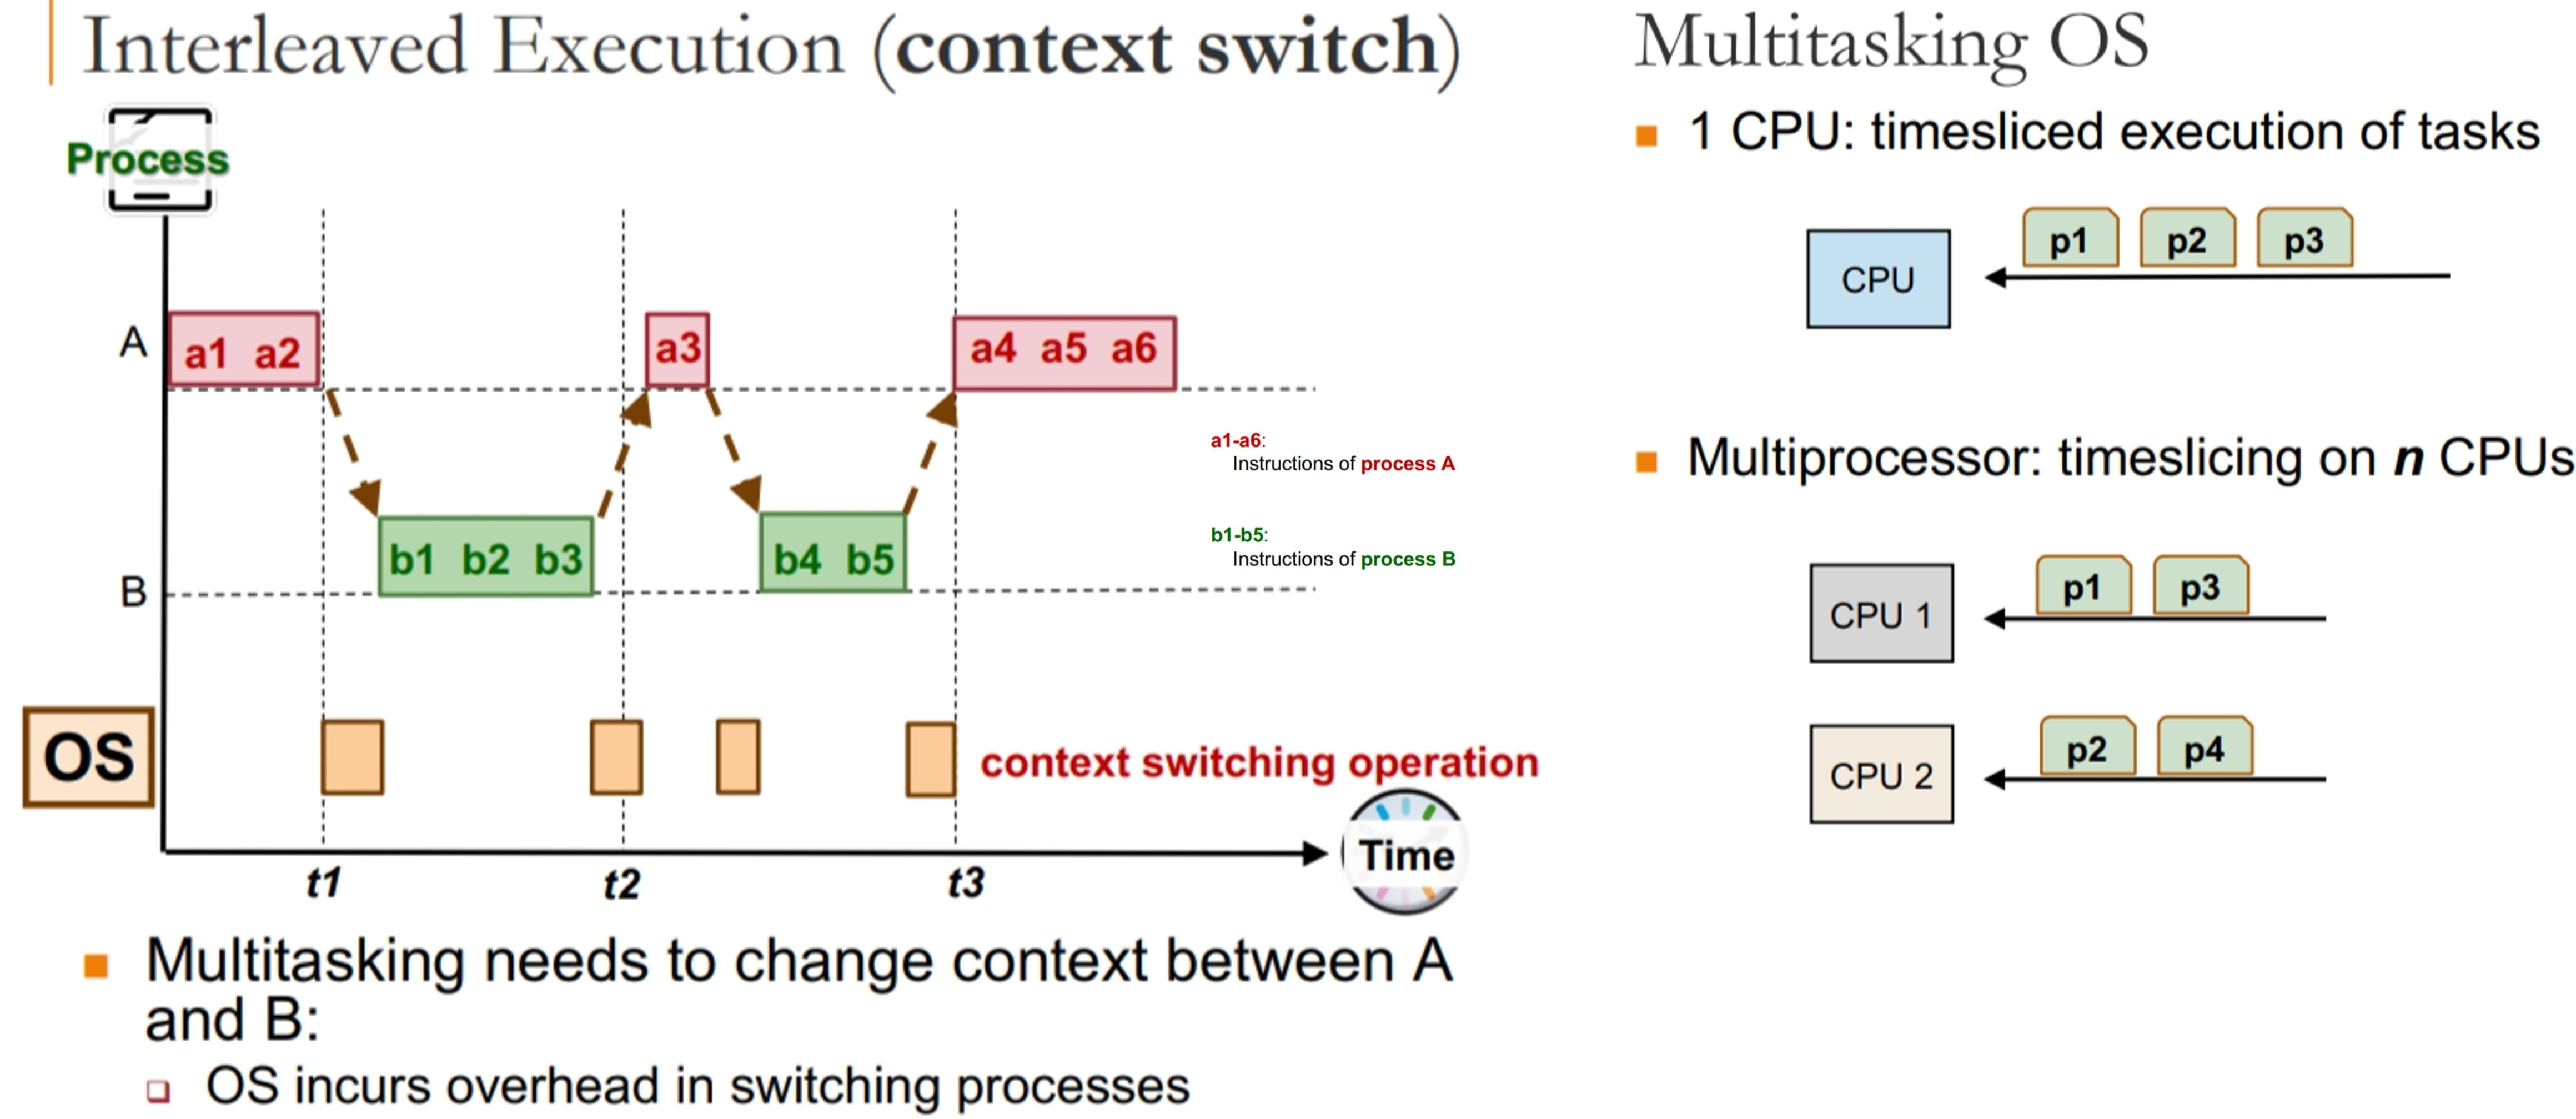
\includegraphics[width=1\linewidth]{timeslice}}
\begin{itemize}
\item \textbf{Scheduling a Process}: \\
1. Scheduler triggered (OS takes over) \\
2. If Context Switch needed, save context, place on blocked/ready queue. \\
3. Pick suitable process $P$ to run base on scheduling algo. \\
4. Setup context for $P$. \\
5. Let process $P$ run.
\end{itemize}

\null \null \null \null \null \null
\null \null \null \null \null \null
\null \null \null \null \null \null
\columnbreak

\section{Scheduling in Batch Systems}
\textbf{Environment}: No user interaction, non-preemptive scheduling predominant. \\
Scheduling algoritms generally easier to understand and implement, with variants and improvements for other type of system. \\
\textbf{Criteria}: Turnaround time (related to waiting time, time spent waiting for CPU). Throughput. CPU utilization.

\subsection{Batch Systems Scheduling Algorithms}
\subsection{FCFS: First-Come First-Served}
\begin{itemize}
\item Tasks stored on \textbf{FIFO queue based on arrival time}.
\item Pick first task in queue to run until done / blocked. Blocked task removed from FIFO queue, when ready, place at back of queue ("newly arrived").
\item \textbf{Evaluation}: \\
- \textit{No starvation}. (Every task eventually processed) \\
- \textit{Covoy Effect}. (CPU-Bound followed by IO-Bound tasks heavily inefficient.) Simple reordering can reduce average waiting time.
\end{itemize}

\subsection{SJF: Shortest Job First (Nonpreemptive)}
\begin{itemize}
\item Select task with \textbf{smallest total CPU time}.
\item Need to know total CPU time for task in advance. \\
- Possible to guess future CPU time by previous CPU-bound phases. 
\end{itemize}
\centerline{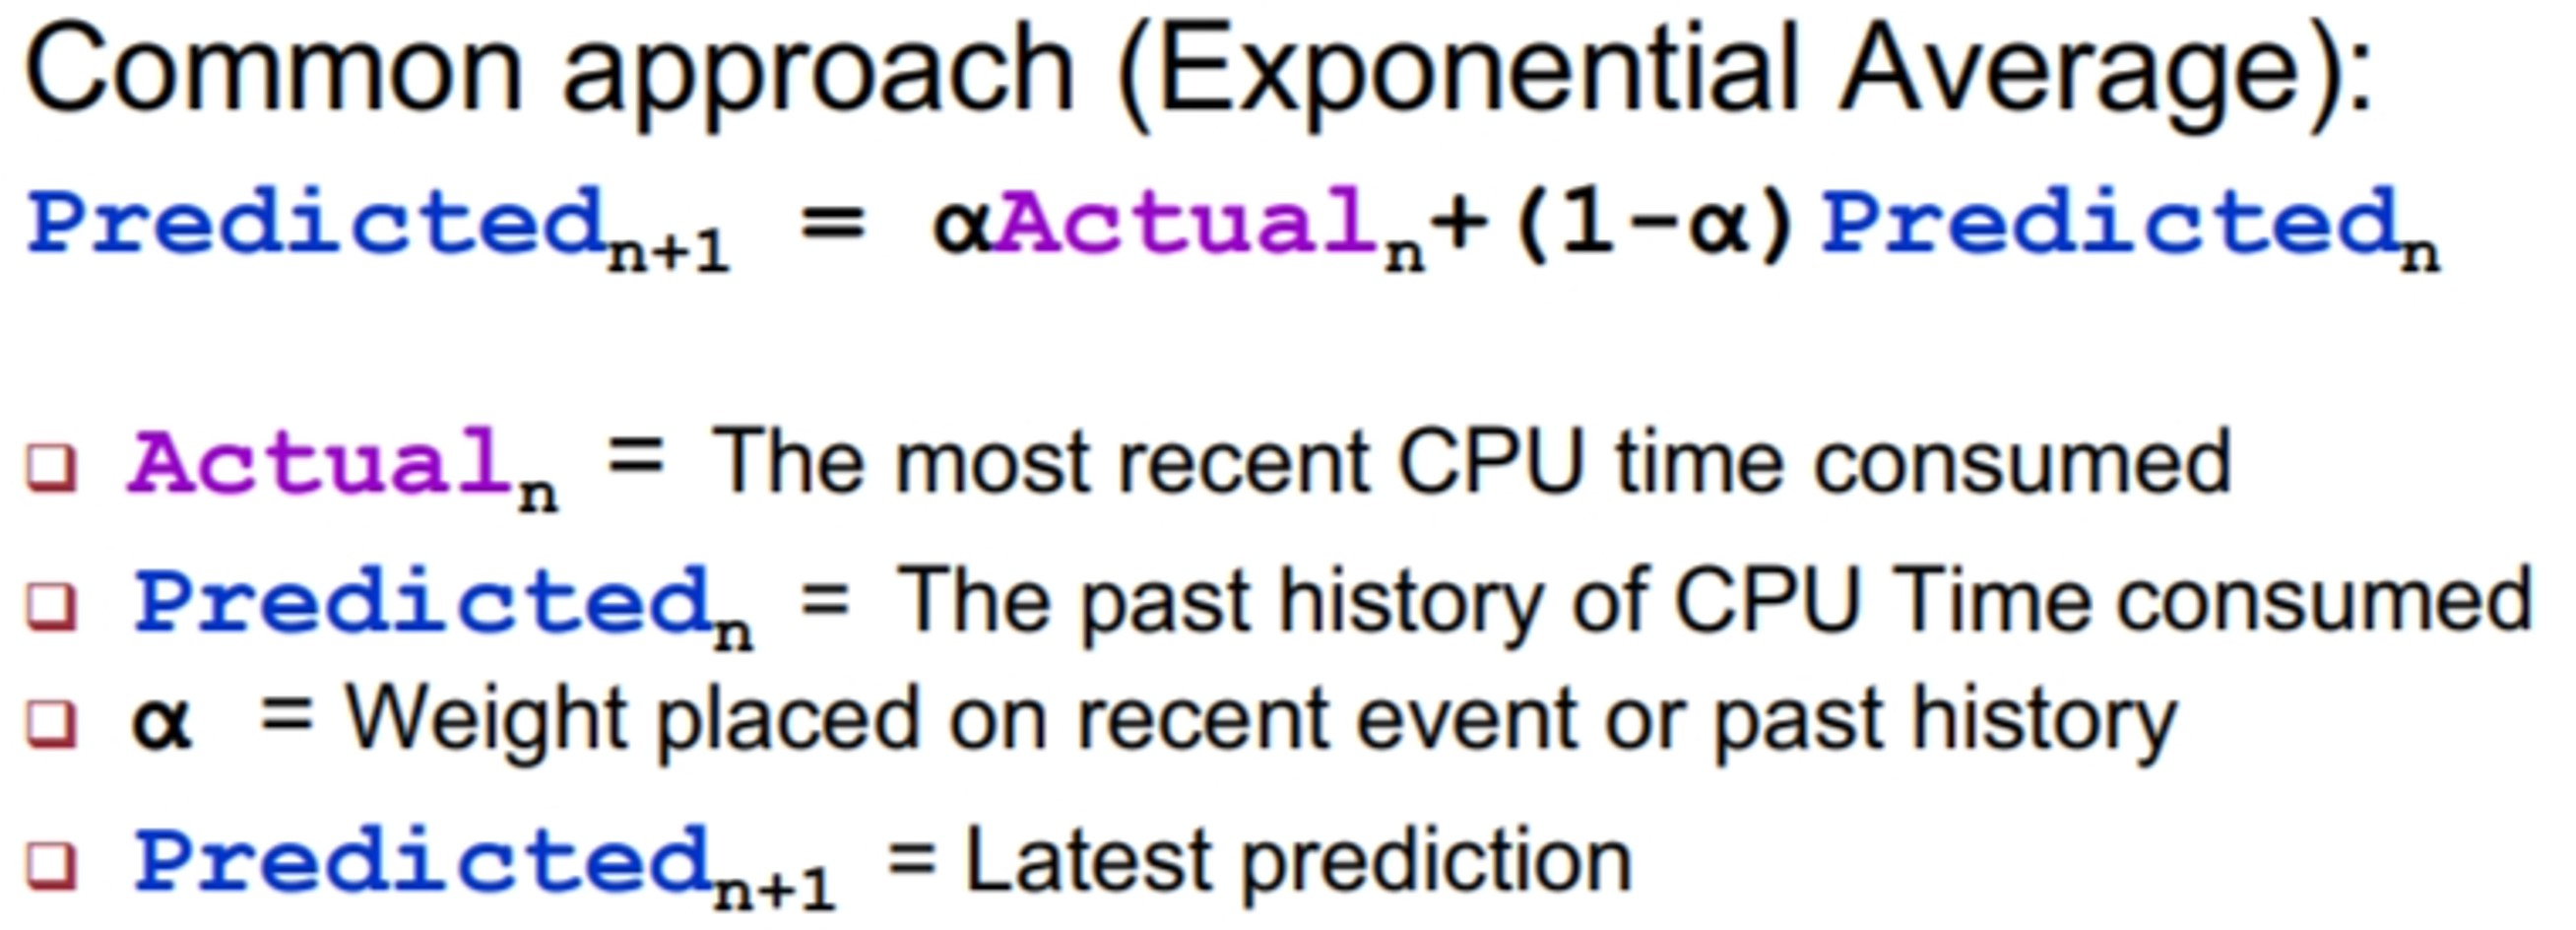
\includegraphics[width=0.6\linewidth]{exponentialAverage}}

\begin{itemize}
\item \textbf{Evaluation}: \\
- \textit{Starvation Possible} (Biased towards short jobs)
- \textit{Minimize average waiting time}.
- Optimal only when all jobs available simultaneously.
\end{itemize}

\subsection{SRT: Shortest Remaining Time Next (Preemptive)}
\begin{itemize}
\item \textbf{Preemptive ver of SJF}. \\
- Scheduler chooses process whose remaining run time is shortest.
\item When new job arrives, total time compared to current process' remaining (or expected) time.
\end{itemize}

\subsection{Batch System Scheduling Examples}
\centerline{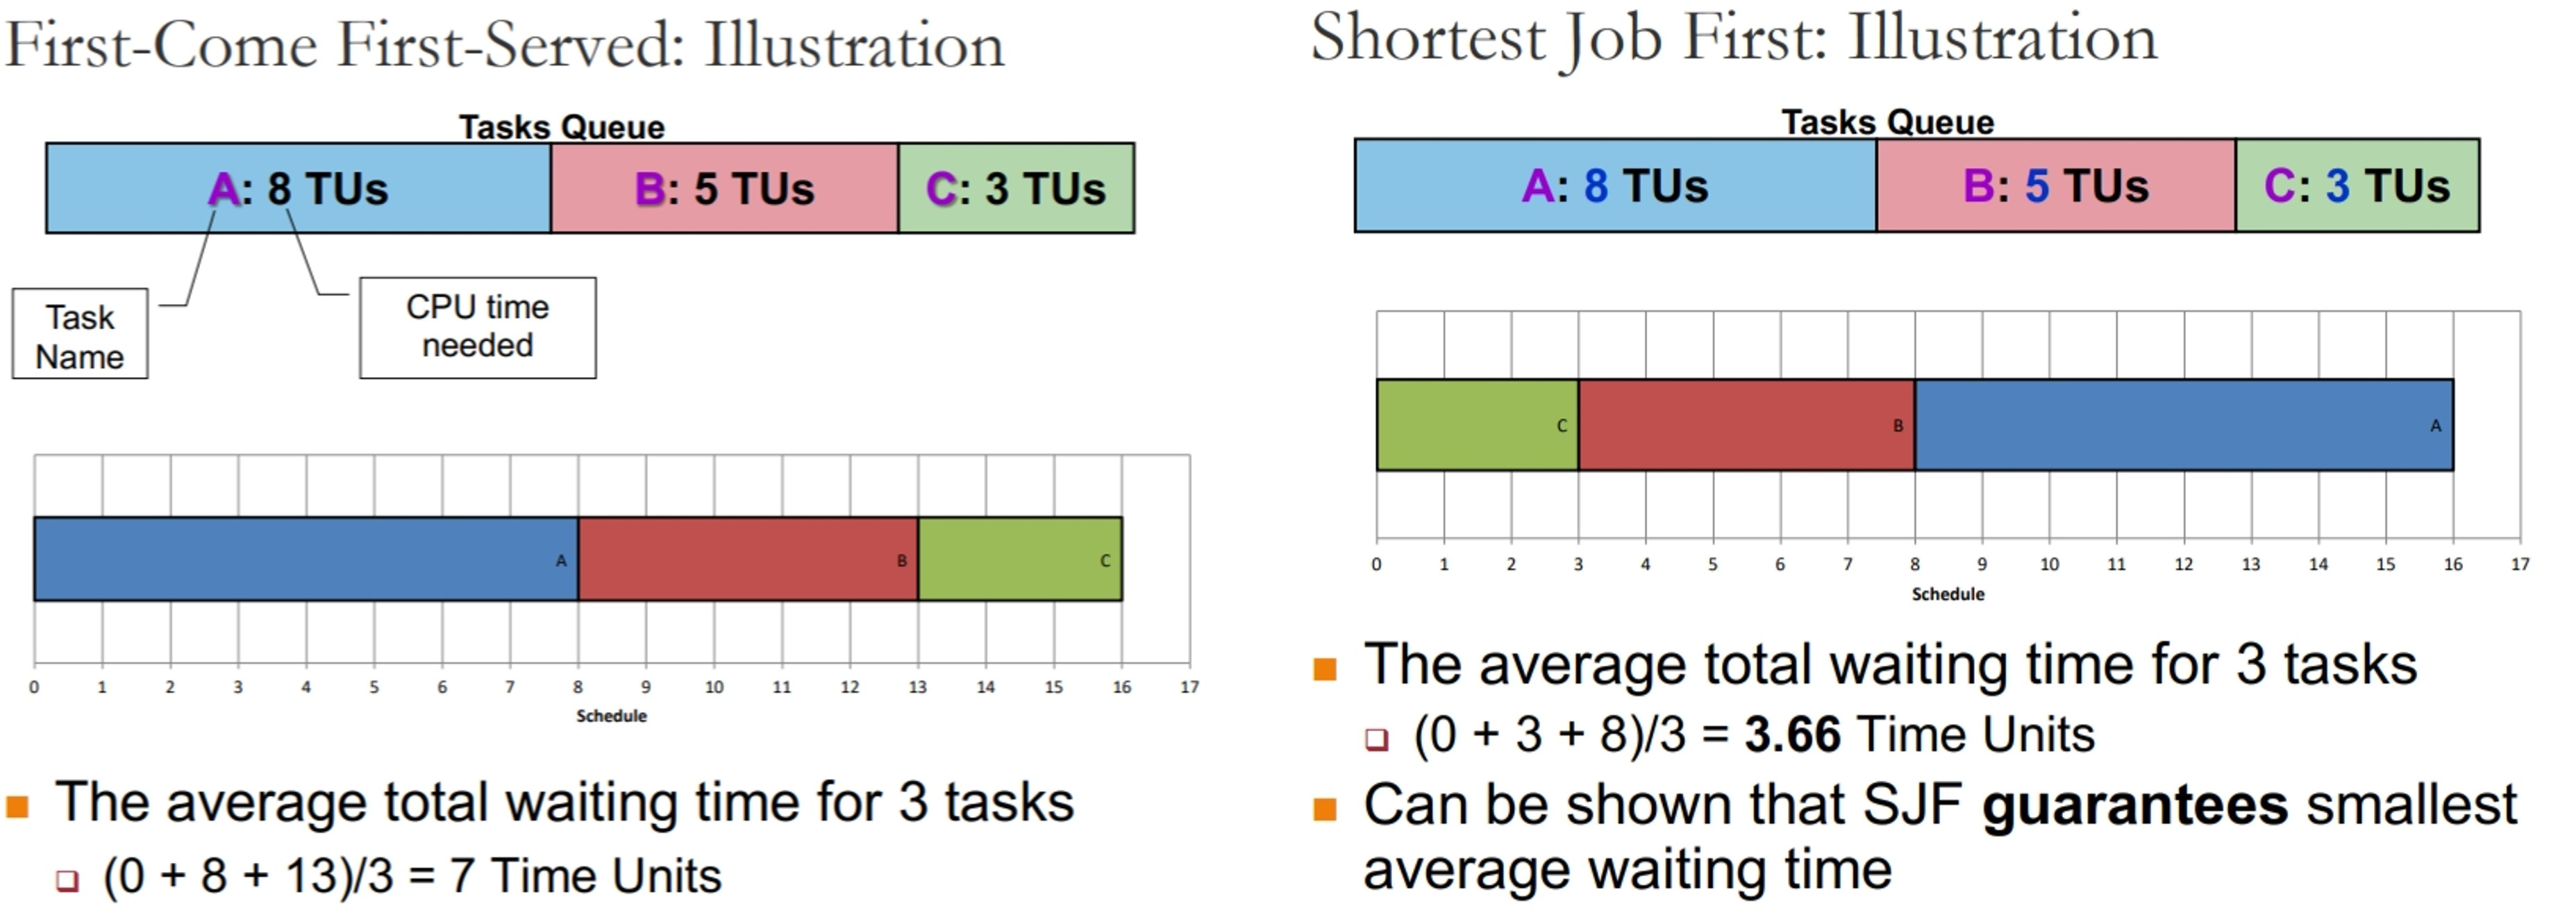
\includegraphics[width=1\linewidth]{batchScheduling}}

\null
\columnbreak

\section{Scheduling in Interactive Systems}
\textbf{Criteria}: Response time (time btwn request \& response). Predictability (Less variation in response time). \\
\textbf{Environment}: User interaction. Preemptive scheduling used to ensure good response time. Scheduler needs to run periodically. \\
\textbf{Ensuring Periodic Scheduler}: Use timer \textbf{interrupts} (based on hardware clock). OS ensures timer interrupt cannot be intercepted by any other program. Interrupt handle \textbf{invokes scheduler}.
\begin{itemize}
\item \textbf{ITI: Interval of Timer Interrupt}: Timing Interval that interrupt happens, and OS scheduler triggered. Typical values (1ms - 10ms).
\item \textbf{Time Quantum}: Execution duration given to each process, constant / variable. Must be multiples of ITI. Typical values (5ms - 100ms).
\end{itemize}
\centerline{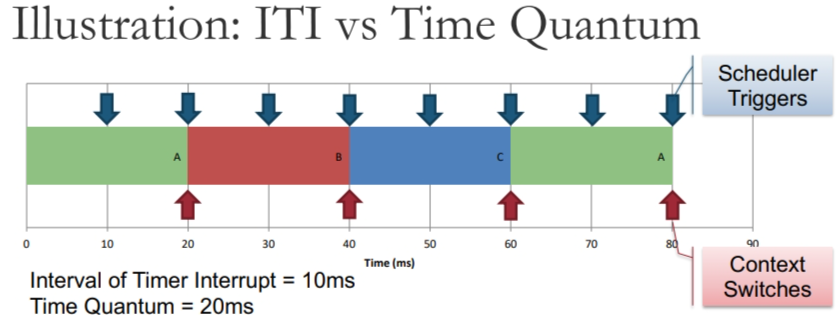
\includegraphics[width=0.8\linewidth]{ITI}}

\subsection{Interactive Systems Scheduling Algorithms}
\subsection{RR: Round Robin}
\begin{itemize}
\item Preemptive ver. of FCFS.
\item \textbf{Tasks stored in FIFO queue}. Each process assigned time quantum, if still running at end, CPU preempted, given to another process. Task placed at end of queue to wait for another turn.
\item \textbf{Response time guarantee}: $n$ tasks, $q$ quantum. Time before task gets CPU bounded by $(n-1)q$.
\item \textbf{Evaluation}: \\
- Setting quantum too short cause many process switches, lower CPU efficiency \\
- Too long quantum causes poor response to short interactive requests.
\end{itemize}

\subsection{Priority Scheduling: Priority Based}
\begin{itemize}
\item Each process assigned a priority, runnable process with highest priority p allowed to run. \\
- \textbf{Preemptive ver.}: Higher p. process can preempt running low p. process. \\
- \textbf{Non-preemptive ver.}: Late high p. process wait for next scheduling.

\item \textbf{Evaluation}: \\
- \textbf{Possible Starvation}: High p. process may hog CPU. \\
To prevent this, scheduler may \textbf{decrease priority} of currently running process at each clock tick (clock interrupt). Or, give some max time quantum, when used up, allow next in line to run. \\
- \textbf{Priority Inversion}: When lower priority task preempts higher priority task. (If lower priority task locks some resource, e.g. file, gets switched, higher priority task cannot run)
\end{itemize}

\columnbreak

\subsection{MLFQ: Multi-Level Feedback Queue}
\begin{itemize}
\item More efficient to give CPU-bound process large quantum once in a while, rather than small quanta frequently to reduce swapping. Also, giving all processes large quantum means poor response time. \\
Hence, solution to set \textbf{multiple priority queues}.
\item As (CPU-bound) process sinks deeper into priority queues, run less frequently, saving CPU for short, interactive processes.
\item Hence, \textbf{adaptively learn process behavior}, minimize both: \\
- Min. Response time for IO bound processes \\
- Min. Turnaround time for CPU bound processes.
\item \textbf{MLFQ Rules}: \\
- \textbf{Basic Rule}: Higher priority process runs. If same p, run in RR. \\
- \textbf{Priority Setting}: New job given highest priority. If job fully utilize time slice, priority reduced. If job gives up / blocks before time slice finished, priority retained.
\item \textbf{Evaluation}:
- \textbf{Can be gamed}: User typing carriage returns at random every few seconds doing wonders for his response time.
\end{itemize}


\subsection{Lottery Scheduling}
\begin{itemize}
\item Give processes lottery tickets for system resources. When scheduling, chose ticket at random.
\item "All processes equal, some processes more equal." More important processes given extra tickets.
\item \textbf{Evaluation}: \\
- \textit{Responsive}: New process can participate in next lottery. \\
- \textit{Good Control}: Each process can distribute to child processes proportionally w.r.t to need. \\
\end{itemize}

\subsection{Interactive System Scheduling Examples}
\centerline{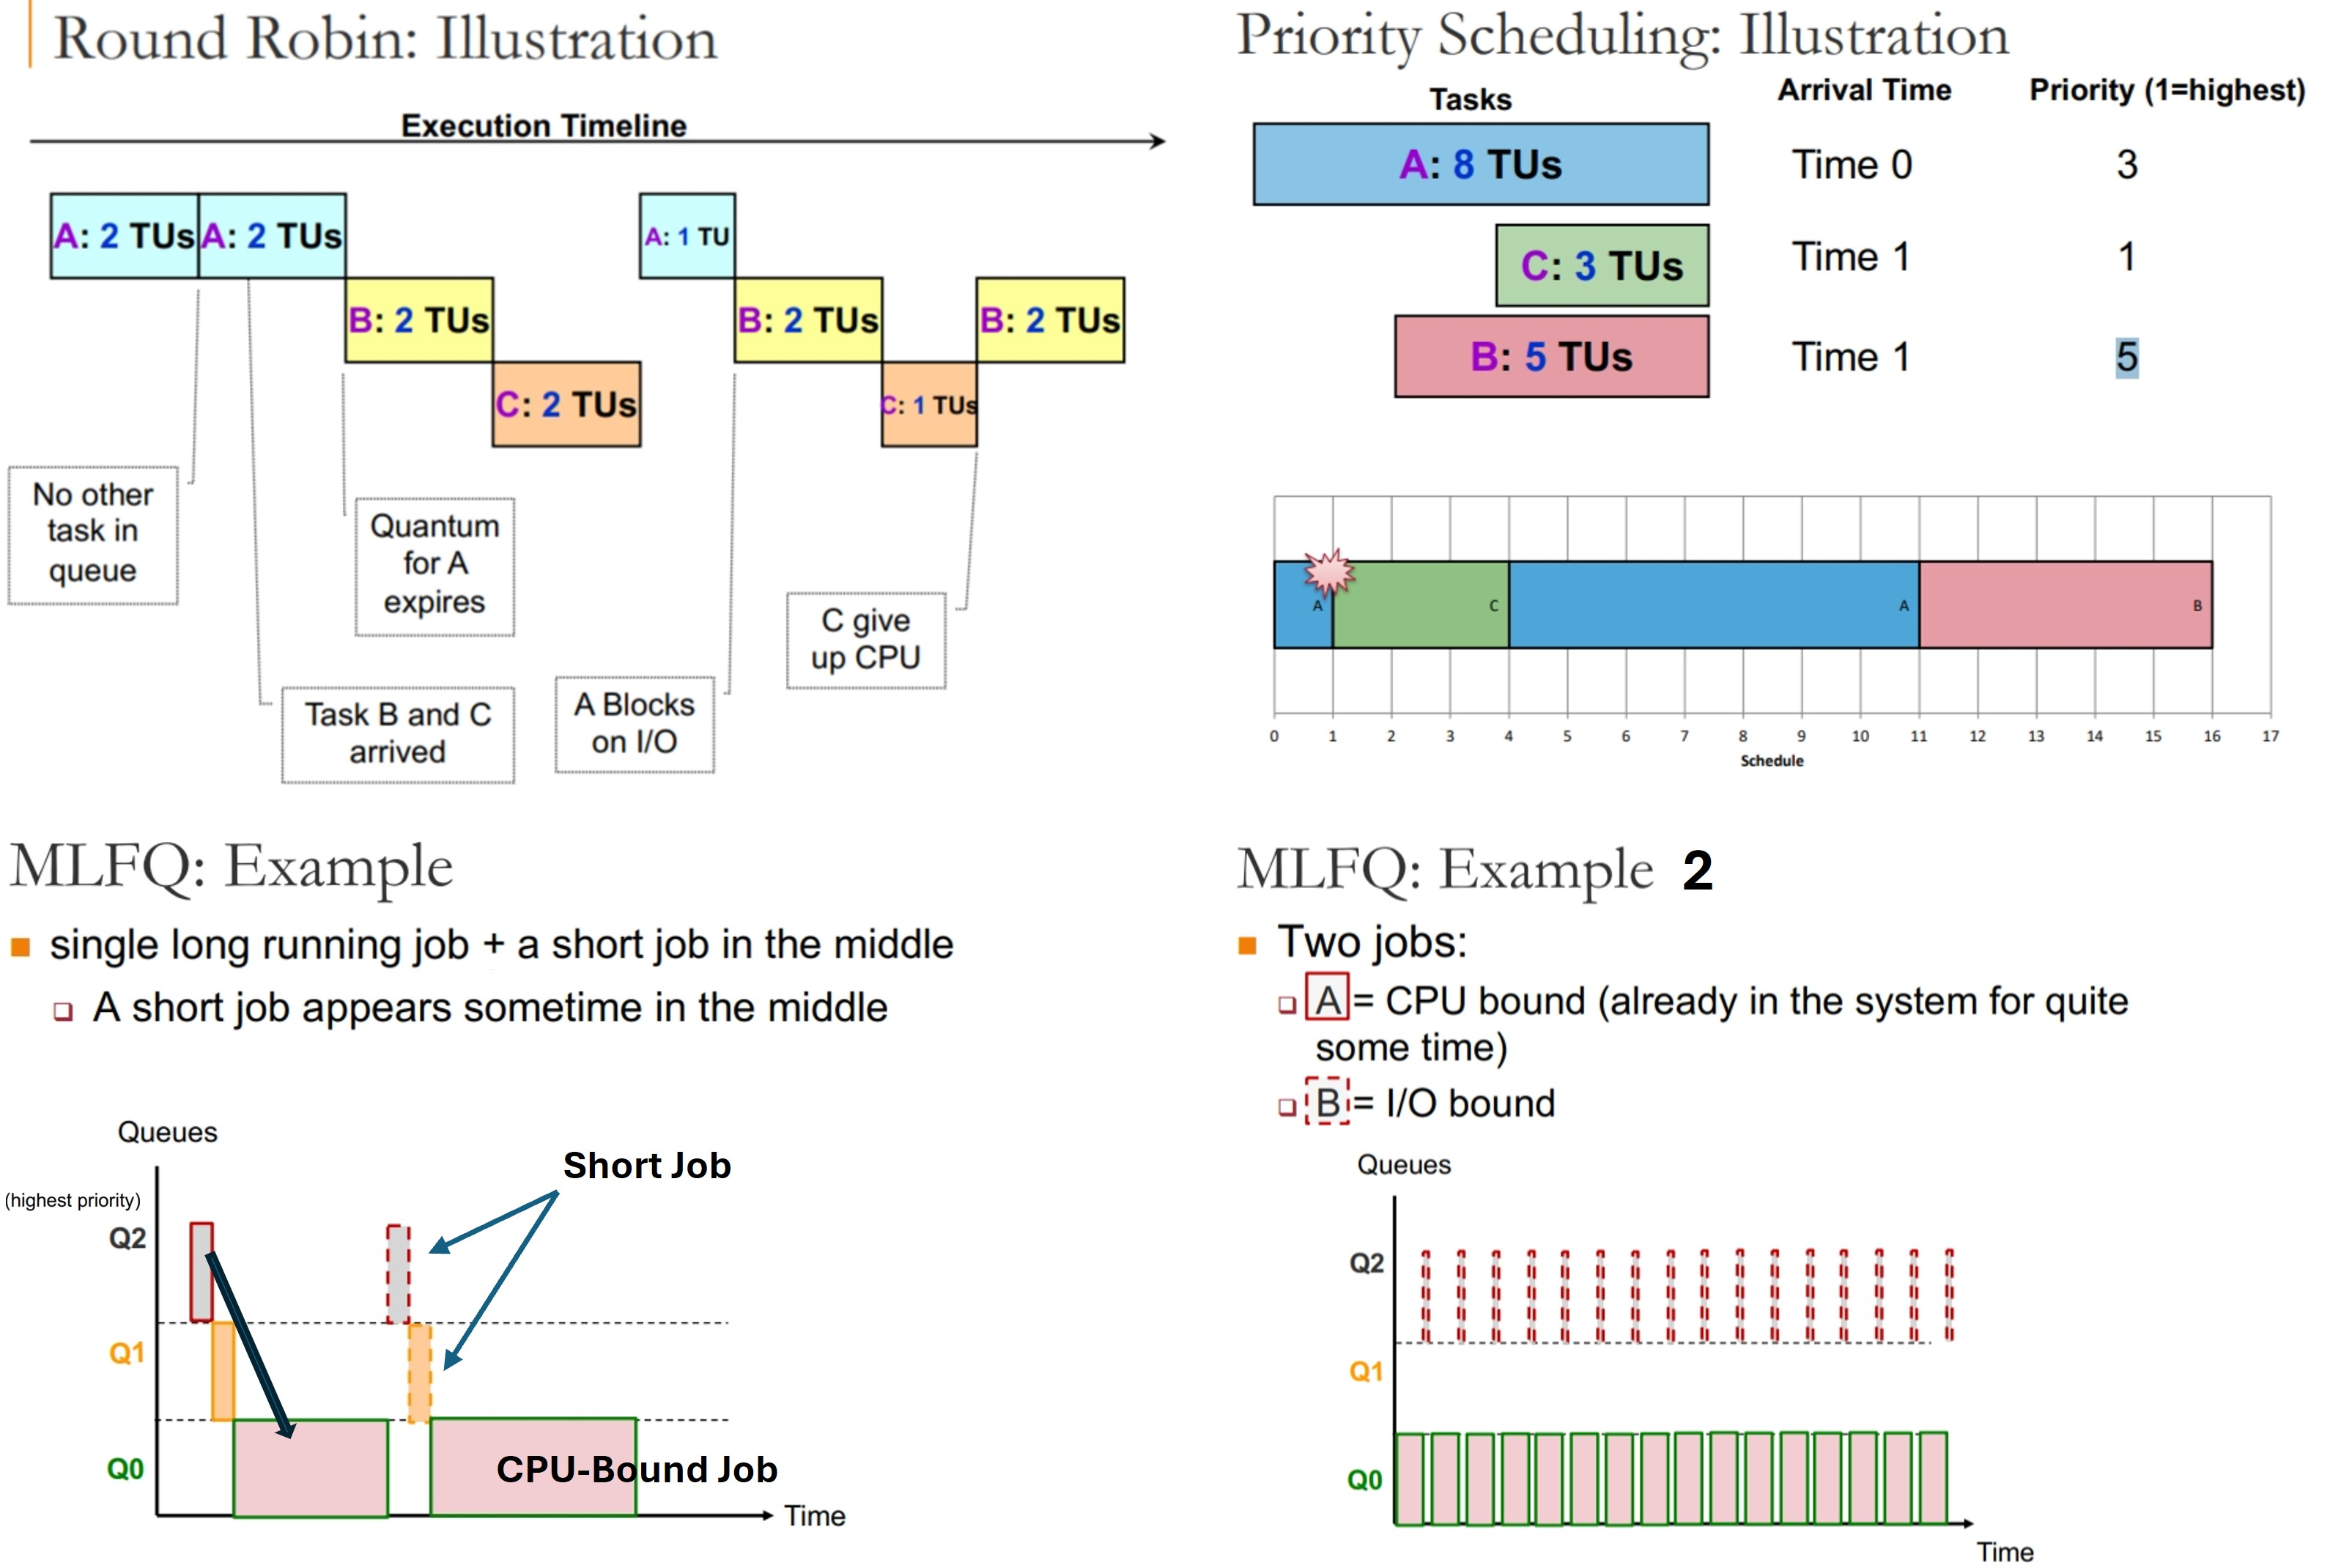
\includegraphics[width=1\linewidth]{interactiveScheduling}}


\subsubsection{Others}
\begin{itemize}
\item \textbf{Shortest Process Next}: Estimate (using calculated aging).
\item \textbf{Guaranteed / Fair-Share Scheduling}: Track CPU usage, run accordingly. Each user gets agreed allocation of CPU.
\end{itemize}



\columnbreak

\section{4.}


















\vfill \null
\columnbreak



~ End.





















































































\end{multicols*}
\end{document}
